\chapter{可测函数}
\label{chap:measurable-functions}

前章给出了两种不同的积分困难。有理数集的示性函数有界，却不能由区间分割得到黎曼积分；越来越窄、越来越高的连续尖峰可以处处趋零，积分却始终为一。前者需要扩大能够积分的函数范围，后者需要控制整个逼近过程。扩大范围不会自动消除第二个困难：即使用新的积分，处处收敛仍不足以保证积分收敛。

本章从“函数值出现在哪些位置，这些位置有多大权重”建立测度和可测函数，再按取值分层构造勒贝格积分。第~\ref{sec:analysis-set-structures}节规定测量范围，第~\ref{sec:analysis-integration-average}节回答怎样累计与计算，第~\ref{sec:measurable-convergence-and-integrals}节研究逼近时怎样保留累计量。最后，第~\ref{sec:measurable-differentiation-recovery}节重新连接微分与积分，分别研究导数何时存在、积分怎样恢复局部数值，以及导数能否恢复整体变化。连续、可测、可积和可微约束的是不同问题，下面每次扩大对象范围时都会重新说明所需条件。

\section{函数的可测性}
\label{sec:analysis-set-structures}

有理数集示性函数只取零和一，累计它的贡献本来只需知道取一的集合有多大。但“集合有多大”需要一套相容的测量规则，不能仅凭两个点的距离决定。本节先分清可以测量的集合与赋予它们的权重，再研究集合极限和零测例外，最后判断函数按取值划出的区域能否留在同一测量范围内。这些基础共同保证下一节的分层累计有明确含义。

\subsection{集合的测量范围与权重}

实轴上的区间长度、有限集合的元素个数和非均匀采样的权重，都在回答集合的累计大小。先规定哪些集合允许参与补集、合并和极限运算，再给这些集合赋值；同一个可测范围仍可以采用不同权重。

\subsubsection{可以测量的集合范围}
\paragraph{补集与可数并下的封闭性}

若能够测量某个条件成立的位置，还应能够测量它不成立的位置；若依次加入可数个区域，也希望最终区域仍可测。因此允许测量的集合族需要对补集和可数并封闭。这些规则只规定测量范围，尚未规定各集合的大小。

\begin{definition}[$\sigma$代数与可测空间]
\label{def:analysis-sigma-algebra}
设$X$为集合。若子集族$\mathcal{A}\subseteq\mathcal{P}(X)$满足
\[
  \begin{gathered}
    X\in\mathcal{A},\\
    A\in\mathcal{A}\Longrightarrow X\setminus A\in\mathcal{A},\\
    A_1,A_2,\ldots\in\mathcal{A}
    \Longrightarrow\bigcup_{n=1}^{\infty}A_n\in\mathcal{A}.
  \end{gathered}
\]
则称$\mathcal{A}$为$X$上的\term{$\sigma$代数}（sigma-algebra）。二元组
$(X,\mathcal{A})$称为\term{可测空间}（measurable space），$\mathcal{A}$中的集合称为
相对于$\mathcal{A}$的\term{可测集合}（measurable set）。
\end{definition}

这些条件还蕴含$\varnothing\in\mathcal A$以及对可数交封闭，后者由De Morgan律得到。采用可数运算，足以表达下面的一列集合或一列函数的极限。若在实轴上既保留区间的通常长度、平移不变性与可数可加性，又要求所有子集都有长度，则会遇到不可测集；本章从明确的可测集合族出发，不把任意子集都当作已经测量。

\paragraph{开集生成的可测范围}

前章的距离已经给出开集。为了让连续函数按输出条件选出的输入范围能够测量，可以至少把全部开集及其可数集合运算纳入；满足这项要求的最小范围称为Borel $\sigma$代数。

\begin{definition}[Borel $\sigma$代数]
\label{def:analysis-borel-sigma-algebra}
在度量空间$(X,d)$中，包含所有开集的最小$\sigma$代数记为$\mathcal{B}(X)$，称为
\term{Borel $\sigma$代数}（Borel sigma-algebra）；其中的集合称为Borel集合。
\end{definition}
“最小”指它包含在每个含有所有开集的$\sigma$代数中。实数上的开区间、闭区间和
单点因而都是Borel集合。度量由此提供一族可测集合，却还没有指定它们的权重；在实数上，
长度测度与把全部权重集中在某一点的测度，都可以定义在同一族Borel集合上。

\subsubsection{集合权重的累计规则}
\paragraph{可数可加的测度}

选定可测范围以后，考虑将集合拆成不重叠的部分。总权重应当等于各部分权重之和，而且这个要求要适用于可数分割，才能与序列极限相容。

\begin{definition}[测度与测度空间]
\label{def:analysis-measure-space}
设$(X,\mathcal{A})$为可测空间。映射$\mu:\mathcal{A}\to[0,\infty]$若满足
$\mu(\varnothing)=0$，并且对任意两两不交的$A_1,A_2,\ldots\in\mathcal{A}$有
\[   \mu\left(\bigcup_{n=1}^{\infty}A_n\right)   =   \sum_{n=1}^{\infty}\mu(A_n). \]
则称$\mu$为\term{测度}（measure）。上述等式称为可数可加性，三元组
$(X,\mathcal{A},\mu)$称为\term{测度空间}（measure space）。
\end{definition}
定义中的非负无穷和约定为有限部分和的上确界，允许结果为$+\infty$：
$\sum_{n\geq1}a_n=\sup_{N\geq1}\sum_{n=1}^N a_n$（$a_n\geq0$）。
前章已用部分和研究一般级数；这里允许非负和为无穷，以表示无限总权重。

有限集合上的计数测度把集合赋值为元素个数；给有限点$x_i$分配质量$w_i\geq0$，则$\mu(A)=\sum_{i:x_i\in A}w_i$。距离仍只比较点的接近程度。例如在$X=\{a,b\}$上固定离散距离$d(a,b)=1$，可以选计数权重$(1,1)$，也可以选非均匀权重$(1,2)$。点列是否收敛不变，函数的加权累计却会改变。取$f(a)=3$、$f(b)=-1$，前一权重累计为$2$，后一权重累计为$1$。下面表中的积分记号先表示这项有限加权累计，正式定义在第~\ref{sec:analysis-integration-average}节给出。

\begin{table}[htbp]
 \centering\small
 \begin{tabularx}{\linewidth}{@{}lXX@{}}
 \toprule
 对象 & 比较或汇总什么 & $X=\{a,b\}$上的例子\\
 \midrule
 度量$d$ & 两点的距离 & $d(a,b)=1$\\
 测度$\mu$ & 集合的权重 & $\mu(\{a\})=1$，$\mu(\{b\})=2$\\
 积分$\int f\,\mathrm d\mu$ & 函数值的加权总量 & $f(a)+2f(b)$\\
 平均 & 总量除以总权重 & $[f(a)+2f(b)]/3$\\
 \bottomrule
 \end{tabularx}
 \caption{距离与权重的不同职责。固定同一个距离仍可选择不同测度；只有总权重为$1$时，积分本身才直接是平均。}
 \label{tab:analysis-metric-measure-integral}
\end{table}

若可测集合$A\subseteq B$，将$B$分为不交的$A$与$B\setminus A$，便有$\mu(B)=\mu(A)+\mu(B\setminus A)\geq\mu(A)$。这是测度的单调性，不依赖函数积分。可数次可加还推出$\mu(\bigcup_n A_n)\leq\sum_n\mu(A_n)$：将每个$A_n$中此前已经出现的点去掉，就得到不交分解。

\paragraph{区间长度与勒贝格测度}

在实轴上，用长度覆盖一个集合可以先给出“最多需要多少长度”的上界。具体地，对任意$E\subseteq\mathbb R$定义外测度
\[
 m^*(E)=\inf\left\{\sum_{j=1}^{\infty}(b_j-a_j):
 E\subseteq\bigcup_{j=1}^{\infty}(a_j,b_j)\right\}.
\]
这里比较所有可数开区间覆盖的总长度，取下确界是为了收紧覆盖造成的多余长度。外测度能用于所有子集，但对任意不交子集还不能直接保证相加。勒贝格可测集合要求分割任何集合时不改变外测度的累计：$A$可测是指对每个$E\subseteq\mathbb R$都有
$m^*(E)=m^*(E\cap A)+m^*(E\setminus A)$。这些$A$构成$\sigma$代数，$m^*$在其上的限制是测度，区间的测度为通常长度，零测集的子集也都已纳入可测范围；这项测度称为勒贝格测度。构造中封闭性与可数可加性的完整证明见测度论教材\scite{math-folland1999real}

本章用$m$或$\mathrm dx$表示一维勒贝格测度，用$m_d$或$\mathrm d\bm x$表示$d$维体积测度。它们的可测集合族都包含Borel集合，实轴上的勒贝格测度是Borel长度测度的完备化。单点长度为零，可数点集也为零；区间可以有正长度，因为可数可加性只允许可数分割，不能把不可数多个单点的权重作为一项可数和。高维版本从矩形覆盖出发，保留同一测量思路。

\subsection{测量中的极限与零测例外}

逐次扩大或缩小区域是积分逼近的基础。下面先检查测度能否传到集合极限，再说明哪些例外不影响累计，以及它们的子集是否也已经进入可测范围。

\subsubsection{集合变化后的测度}
\label{sec:analysis-set-measure-continuity}
\paragraph{递增集合的累计极限}

可测范围逐步扩大时，已经纳入的权重会不会在极限中丢失？后面的积分逼近会将取值层对应的集合逐步扩大，因此先检查这种集合极限。记
$A_n\uparrow A$表示$A_n\subseteq A_{n+1}$且$A=\bigcup_nA_n$；
记$A_n\downarrow A$表示$A_n\supseteq A_{n+1}$且$A=\bigcap_nA_n$。
这两种集合极限分别保留所有最终进入的点、所有始终没有被排除的点。
可数可加性给出相应的测度连续性。以下各集合均属于可测集合族$\mathcal A$。若
$A_1\subseteq A_2\subseteq\cdots$且$A=\bigcup_nA_n$，令
$B_1=A_1$、$B_n=A_n\setminus A_{n-1}$，则$B_n$两两不交且
$A_n=\bigcup_{k=1}^nB_k$。因此
\[
  \mu(A)
  =
  \sum_{k=1}^{\infty}\mu(B_k)
  =
  \lim_{n\to\infty}\mu(A_n).
\]
这里的极限就是非负有限部分和的上确界，允许为无穷，不依赖函数积分。
例如实轴上的$A_n=(0,1-1/n)$递增到$(0,1)$，其长度$1-1/n$也趋于$1$；
端点$1$虽然从未进入集合，但集合的极限仍有完整的单位长度。

\paragraph{递减集合的有限性条件}

若$A_1\supseteq A_2\supseteq\cdots$且$\mu(A_1)<\infty$，令$A=\bigcap_nA_n$。
对递增集合$A_1\setminus A_n$应用上一结论，得到
\[
 \mu(A_1)-\mu(A)
 =\mu(A_1\setminus A)
 =\lim_n\mu(A_1\setminus A_n)
 =\mu(A_1)-\lim_n\mu(A_n).
\]
所有相减项均有限，故$\mu(A)=\lim_n\mu(A_n)$。
例如$[0,1/n]\downarrow\{0\}$且长度趋于$0$。
递减情形需要$\mu(A_1)<\infty$：
若每个$A_n$的测度都为无穷，就不能通过“无穷减无穷”得到结论。例如Lebesgue测度下
$A_n=(n,\infty)$递减到空集，但每个$A_n$的测度仍为无穷。


图~\ref{fig:vol1-add-nested-set-limits}对照上述三列集合。前两列的长度能够传到极限，第三列的点虽然全部移走，每一步仍有无穷长度，说明递减集合的有限测度条件不能省略。
\begin{figure}[!htb]
  \centering
  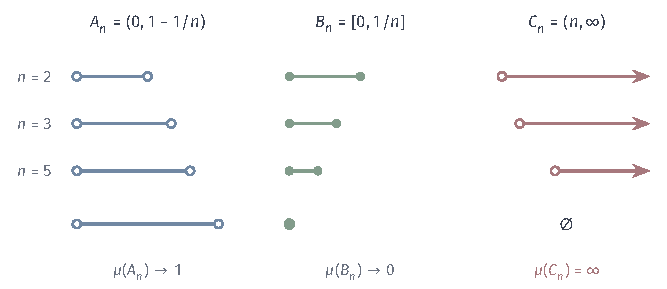
\includegraphics[width=112mm]{figures/01-mathematical-preliminaries-upper/01-mathematical-language-combinatorics-analysis-optimization/tikz/comprehension-additions/nested-set-limits.pdf}
  \caption{实轴上三种嵌套集合，依次画$n=2,3,5$及极限集合，均使用Lebesgue测度。左列$A_n$递增到$(0,1)$，中列$B_n$递减到单点$\{0\}$；右列$C_n=(n,\infty)$递减到空集，每一项的测度却仍为无穷。空心、实心端点分别表示不包含、包含。各列仅在本列内共用坐标尺度。}
  \label{fig:vol1-add-nested-set-limits}
\end{figure}

\subsubsection{可以忽略的例外范围}
\paragraph{零测集与几乎处处}

这种权重允许某些非空集合的大小为零。讨论积分和函数极限时，这些集合上的例外
往往不影响总量；“几乎处处”就是把这种可忽略性说清楚。
\begin{definition}[零测集与几乎处处]
\label{def:analysis-null-set-almost-everywhere}
在测度空间$(X,\mathcal{A},\mu)$中，若$N\in\mathcal{A}$且$\mu(N)=0$，称$N$为
\term{零测集}（null set）。若存在这样的$N$，使某性质对每个$x\in X\setminus N$
成立，称该性质$\mu$-\term{几乎处处}（almost everywhere，简写为a.e.）成立。
\end{definition}
这里不要求例外集合为空，而是要求它包含在一个可测的零测集中。换用另一个测度后，
原来的例外可能不再可忽略。例如单点在长度测度下为零，在计数测度下却有质量$1$。

\paragraph{零测子集与测度完备化}

还会遇到另一项要求：一个集合既然没有权重，它的任何子集也应能被赋予零权重。
这项要求并非由可数可加性自动保证，因此需要单独说明。
\begin{definition}[完备测度空间]
\label{def:analysis-complete-measure-space}
若测度空间$(X,\mathcal{A},\mu)$中每个零测集$N$的任意子集$E\subseteq N$都属于
$\mathcal{A}$，称该测度空间完备。此时由测度的单调性还有$\mu(E)=0$。
\end{definition}
把可测零测集的所有子集加入原$\sigma$代数，并相应扩展测度，称为测度空间的完备化。
具体地，令
\[
 \begin{aligned}
 \overline{\mathcal A}
 &=\left\{A\cup E:
     \begin{array}{l}
       A,N\in\mathcal A,\quad \mu(N)=0,\\
       E\subseteq N
     \end{array}\right\},\\
 \bar\mu(A\cup E)&=\mu(A).
 \end{aligned}
\]
若同一集合还有表示$A'\cup E'$，则$A\setminus A'$与$A'\setminus A$
都包含在可测零测集中，其本身可测且测度为零，由有限可加性得$\mu(A)=\mu(A')$，
赋值不依赖表示。
取补集时，可把$A\cup E$的补集写成
$(X\setminus(A\cup N))\cup(N\setminus(A\cup E))$；
第二项仍是零测集的子集。取可数并时，可测部分取并，例外部分包含在零测集的可数并中，
因而$\overline{\mathcal A}$是$\sigma$代数。对两两不交的$A_j\cup E_j$，
其可测部分$A_j$也两两不交，$\bar\mu$的可数可加性随即由$\mu$继承。
若$\bar\mu(A\cup E)=0$，则$A\cup E$包含在原可测零测集$A\cup N$中；
它的任意子集已被纳入$\overline{\mathcal A}$，所以扩展后的空间完备。

一个有限例子能看清增加了什么。取$X=\{a,b,c\}$、
$\mathcal A=\{\varnothing,\{a,b\},\{c\},X\}$，令$\mu(\{a,b\})=0$、
$\mu(\{c\})=1$。原来不能单独测量$\{a\}$；完备化把$\{a\}$、$\{b\}$
及其与$\{c\}$的并纳入，得到全部子集，并把新增零测子集赋值为零。
实数上的Lebesgue测度空间则是Borel长度测度空间的完备化；新增的集合仍保持相容的长度。
这里的完备性处理零测集的子集，不同于前章中
“柯西数列不会逃出空间”的完备性。

\subsection{函数的可测判定与保持}

测度只给集合赋权。要累计函数，就要知道函数取某些值的输入集合能否测量。下面先把输出条件转成输入原像，再检查连续映射、函数运算和点态极限能否保持这种相容性。

\subsubsection{按函数取值划分区域}
\paragraph{阈值集合与原像条件}

以集合$\{x:f(x)>a\}$为例，它记录超过阈值$a$的全部输入。若这样的集合不在允许测量的范围内，便无法为这一层赋权；因此先用原像条件规定函数与可测范围的相容性。

可测性说的是函数与这些测量范围是否相容：对输出值提出一个可测的条件，满足条件的
输入也应组成可测集合。这里需要的是集合的原像，并不要求函数有逆函数。
\begin{definition}[可测函数]
\label{def:analysis-measurable-function}
给定可测空间$(X,\mathcal{A})$与$(Y,\mathcal{B})$。若映射$f:X\to Y$满足
\[
  B\in\mathcal{B}\quad\Longrightarrow\quad
  f^{-1}(B)=\{x\in X:f(x)\in B\}\in\mathcal{A},
\]
则称$f$为从$(X,\mathcal{A})$到$(Y,\mathcal{B})$的\term{可测函数}
（measurable function）。对取值于$\mathbb{R}$或$\overline{\mathbb{R}}=[-\infty,\infty]$
的函数，目标空间取Borel $\sigma$代数；此时可测性等价于
\[
  \{x\in X:f(x)>a\}\in\mathcal{A}
  \qquad\text{对每个 }a\in\mathbb{R}\text{成立}.
\]
\end{definition}
阈值条件之所以足够，是因为这些半直线能生成目标空间的Borel $\sigma$代数，而原像
保持补集与可数并。它保证按函数值分层得到的集合都能取得测度。可测性依赖指定的
$\sigma$代数，并不依赖这些集合具体有多大权重。例如在$X=\{a,b\}$上只允许
$\mathcal{A}=\{\varnothing,X\}$时，$f(a)=0$、$f(b)=1$不可测：阈值$1/2$选出
$\{b\}$，不在$\mathcal{A}$中。把$\mathcal{A}$改为所有子集后，同一个函数就可测。

\paragraph{连续函数与不连续可测函数}

连续性比较输入与输出的距离，本身不以可测性为先决条件。若两端采用Borel $\sigma$代数，连续映射自动可测，因为开集的原像仍是开集；若任意指定其他$\sigma$代数，则不能只凭连续性保证可测。反向也不成立。

例如$[0,1]$上的有理数集示性函数$\mathbb I_{\mathbb Q\cap[0,1]}$可测，因为有理数集是可数个单点的并；它却在每一点都不连续，因为每个邻域同时有有理数和无理数。这里扩大的是允许按取值测量的函数范围，没有同时得到连续或可积的保证。

\subsubsection{运算与极限后的可测性}
\paragraph{函数运算与复合}

若$f,g$是可测实函数，则$(f,g)$的可测矩形原像是两个可测原像的交，而实平面开集能写成可数个有理端点矩形的并。因此$(f,g)$作为到$\mathbb R^2$的映射可测；再复合连续的加法、乘法、绝对值、最大最小等运算，所得函数仍可测。商$f/g$还要求分母非零，或者明确规定零点上的取值。扩展实函数的运算要另外排除$+\infty-\infty$等未定义情形。

一般地，可测映射的复合仍可测，因为$(h\circ f)^{-1}(B)=f^{-1}(h^{-1}(B))$。这里须让中间空间采用同一个$\sigma$代数；只知道某个实函数是勒贝格可测，不能不检查中间可测范围就与任意可测映射复合。

\paragraph{点态极限与上下包络}

这些极限的可测性可以直接回到集合运算，而不依赖尚未建立的积分定理。对可测实函数列，
\begin{align*}
 \{x:\sup_n f_n(x)>a\}&=\bigcup_n\{x:f_n(x)>a\},\\
 \{x:\inf_n f_n(x)<a\}&=\bigcup_n\{x:f_n(x)<a\}.
\end{align*}
因此上确界、下确界可测；再用
$\liminf_n f_n=\sup_N\inf_{n\geq N}f_n$，得到下极限可测，逐点极限存在时就是它。

可数上下包络还会用于积分极限：它们把一列可能振荡的函数改成有序逼近，且始终留在原来的可测函数范围内。与前章相比，连续函数的逐点极限可能失去连续性，可测函数类则保留这一点态极限性质。

可测性仍依赖指定的集合族。例如在$\mathbb R$上采用通常距离，却只允许$\{\varnothing,\mathbb R\}$可测，连续函数$f(x)=x$就不对Borel目标可测，因为$(0,1)$的原像未被允许测量。后面除非另有说明，欧氏空间采用勒贝格测度及其可测范围，实函数的目标采用Borel集合族。

\section{函数的积分与可积性}
\label{sec:analysis-integration-average}

可测性保证函数按取值分层后，各层都能测量；它还没有规定如何把无限多个取值累计起来。本节从有限分层的加权和出发，经非负逼近构造积分，再分开正负部分判断积分是否有意义且有限。建立积分以后，先与前章的黎曼积分核对共同范围，再推广分步计算和坐标换元。这样可以区分积分的定义、存在条件和计算方法。

\subsection{一般函数积分的构造}

有限分层可以直接计算，任意非负函数可以从下方逼近，有符号函数则还要处理正负贡献相消。下面按这三个对象范围构造积分，后一步只使用此前已经建立的运算性质。

\subsubsection{有限分层的直接累计}
\paragraph{简单函数的加权求和}

只取有限多个值的函数，其累计量可以按取值乘集合权重求和。这不要求每一层都是区间；有理数集这样分散的集合也可以成为一层。

\begin{definition}[简单函数及其积分]
\label{def:analysis-simple-function-integral}
在可测空间$(X,\mathcal{A})$上，只取有限多个实数值的可测函数称为
\term{简单函数}（simple function）。非负简单函数可以表示为
\[   s(x)=\sum_{j=1}^{m}a_j\mathbb{I}_{A_j}(x),   \qquad a_j\in[0,\infty),\quad A_j\in\mathcal{A}, \]
其中$A_j$两两不交，$\mathbb{I}_{A_j}$在$A_j$上取$1$、其余处取$0$。
给定测度$\mu$，其积分定义为
\begin{equation}
  \int_X s\,\mathrm{d}\mu
  =
  \sum_{j=1}^{m}a_j\mu(A_j).
\label{eq:analysis-simple-integral}
\end{equation}
约定$0\cdot\infty=0$，并允许积分取$+\infty$。
\end{definition}

\paragraph{分层表示与共同细分}

同一个简单函数可能有不同的分组表示；把这些表示按所有取值集合的交集细分成共同的
两两不交集合后，有限可加性给出相同的和，因此式~\eqref{eq:analysis-simple-integral}
不依赖具体表示。
同样的共同细分还给出简单函数的大小关系与非负线性：
若$s\leq t$，则$\int s\leq\int t$；若$\alpha,\beta\geq0$，则
$\int(\alpha s+\beta t)=\alpha\int s+\beta\int t$。
这些结论只涉及同一组可测块上的有限加权和，尚未对一般函数交换极限和积分。

例如对$[0,1]$上的$f(x)=x$，用两段阶梯从下方近似：前半段取$0$，后半段取
$1/2$，其积分为$1/4$。细分成四段并取每段左端点的函数值，积分变成
$(0+1/4+1/2+3/4)/4=3/8$；继续细分，阶梯越来越接近原函数，面积趋于熟悉的$1/2$。
这里每个阶段都只计算有限个“取值$\times$集合长度”，极限才把它们接成一般积分。

\subsubsection{非负函数的逼近累计}
\paragraph{简单函数下逼近与积分上确界}

这一做法不限于区间。每个非负可测函数$f$都能由一列非负简单函数从下方逐点逼近。
对$n\geq1$，一个明确的构造是
\begin{equation}
  s_n(x)
  =
  \sum_{k=0}^{n\,2^n-1}
  \frac{k}{2^n}
  \mathbb{I}_{\{k\,2^{-n}\leq f(x)<(k+1)2^{-n}\}}
  +
  n\mathbb{I}_{\{f(x)\geq n\}}.
\label{eq:analysis-canonical-simple-approximation}
\end{equation}
它先把函数值截断在$n$，再向下舍入到间距为$2^{-n}$的格点。截断高度随$n$增加，
格点也逐次细化，所以$0\leq s_n\leq s_{n+1}\leq f$。若$f(x)<\infty$，当
$n>f(x)$时还有$0\leq f(x)-s_n(x)<2^{-n}$；若$f(x)=+\infty$，则
$s_n(x)=n$。因此$s_n(x)\uparrow f(x)$对每个$x$成立。每个下方阶梯给出一个不超过
真实总量的值；把所有这种值的上界收紧，就得到非负积分。
图~\ref{fig:analysis-simple-integral}把同一构造用于$f(x)=x^2$。等距划分的是
\emph{函数值}，对应的输入区间宽度不必相等；每块绿色面积仍是一个取值乘以
它的原像集合的测度。随着取值间距缩小，下方阶梯留下的空隙逐渐减小。
\begin{figure*}[htbp]
  \centering
  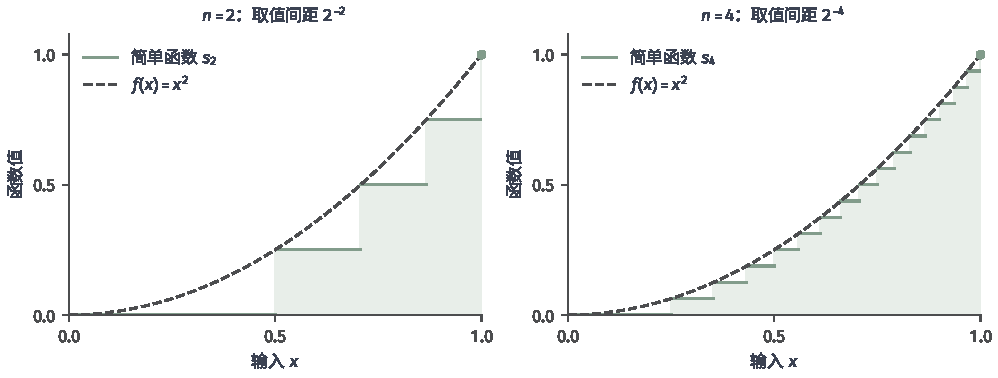
\includegraphics[width=169.0mm]{figures/01-mathematical-preliminaries-upper/01-mathematical-language-combinatorics-analysis-optimization/matplotlib/analysis-simple-integral/figure.pdf}
  \caption{按取值分层的简单函数逼近。两图都使用式~\eqref{eq:analysis-canonical-simple-approximation}的构造，分别取$n=2$和$n=4$；本例中高度截断不起作用。绿色阶梯下的面积是有限加权和，目标曲线下的面积为$1/3$。两图共用坐标尺度。}
 \label{fig:analysis-simple-integral}
\end{figure*}
\begin{definition}[非负函数的Lebesgue积分]
\label{def:analysis-nonnegative-lebesgue-integral}
在测度空间$(X,\mathcal{A},\mu)$上，非负可测函数$f:X\to[0,\infty]$的积分定义为
\begin{equation}
  \int_X f\,\mathrm{d}\mu
  =
  \sup\left\{
    \int_X s\,\mathrm{d}\mu:
    0\leq s\leq f,\ s\text{为简单函数}
  \right\}.
\label{eq:analysis-nonnegative-lebesgue-integral}
\end{equation}
这里允许结果为$+\infty$。
\end{definition}
这个定义按函数值分层而不是把定义域切成小区间，所以能自然处理极限和零测例外。
式~\eqref{eq:analysis-canonical-simple-approximation}给出的阶梯可以用来计算这个
上确界；下面的单调收敛定理说明，任意这样的递增逼近都给出同一个值。

\paragraph{递增逼近与积分保持}

非负积分定义直接保留大小关系：若$0\leq f\leq g$，每个不超过$f$的简单函数
也不超过$g$，所以$\int f\,\mathrm d\mu\leq\int g\,\mathrm d\mu$。
它也继承零测修改不变性。设$N$可测且$\mu(N)=0$，$f,g$可测非负并在$X\setminus N$
相等。任取简单函数$0\leq s\leq f$，去掉$N$上的部分得到
$s\mathbb I_{X\setminus N}\leq g$，且简单函数积分没有改变；取上确界得到
$\int f\leq\int g$，反向同理。这里没有用一般积分的线性，只用了简单函数的有限和。
修改后的函数仍须可测；在未完备测度空间中，不能在零测集上任意修改而省略这项要求。

一种防止总量在逼近中消失的方式，是只让非负贡献逐步增加。它正好对应上面的下方阶梯。记$f_n(x)\uparrow f(x)$表示每个固定$x$处的数列单调增加且趋于$f(x)$；允许忽略零测例外时，例外须包含在同一个可测零测集中。下面把阶梯逼近推广到任意递增的非负可测函数列\scite{math-folland1999real}
\begin{theorem}[单调收敛定理]
\label{thm:analysis-monotone-convergence}
设$f_n,f:X\to[0,\infty]$可测，且$f_n(x)\uparrow f(x)$几乎处处，则
\[   \lim_{n\to\infty}\int_X f_n\,\mathrm{d}\mu   =   \int_X f\,\mathrm{d}\mu. \]
两边都允许取$+\infty$。
\end{theorem}
\begin{proof}
把单调性或收敛关系失效的可测零测集并为$N$，并将$f_n$与$f$在$N$上都改为$0$。
修改后的函数仍可测且积分不变，所以可假定$f_n\uparrow f$逐点成立。由
$0\leq f_n\leq f$，积分序列单调不减且
\[   L:=\lim_{n\to\infty}\int f_n\,\mathrm{d}\mu   \leq\int f\,\mathrm{d}\mu. \]
还需证明反向不等式。任取满足$0\leq s\leq f$的简单函数，将它写为 $s=\sum_{j=1}^m a_j\mathbb{I}_{E_j}$，其中$a_j>0$且$E_j$两两不交。固定 $c\in(0,1)$，定义
\[   E_{j,n}   =   E_j\cap\{x:f_n(x)\geq ca_j\}. \]
由于$f_n\uparrow f$且$f\geq a_j$于$E_j$，有$E_{j,n}\uparrow E_j$。
第~\ref{sec:analysis-set-measure-continuity}节已由可数可加性证明测度对递增集合连续，
故$\mu(E_{j,n})\uparrow\mu(E_j)$。同时
\[   f_n   \geq   c\sum_{j=1}^m a_j\mathbb{I}_{E_{j,n}}, \]
从而
\[   L   \geq   \lim_{n\to\infty}   c\sum_{j=1}^m a_j\mu(E_{j,n})   =   c\int s\,\mathrm{d}\mu. \]
先令$c\uparrow1$，再对所有$0\leq s\leq f$的简单函数取上确界。根据非负积分的定义~\eqref{eq:analysis-nonnegative-lebesgue-integral}， $L\geq\int f\,\mathrm{d}\mu$。与前一不等式合并即得结论。
\end{proof}

非负性避免正负无穷相消，单调性保证已经积累的质量不会在后续消失。定理不要求存在可积的统一上界，也不要求各$\int f_n$有限。

单调收敛已经说明递增逼近怎样保留总量。积分还应继承有限和的两个基本规律：贡献增加时总量不能减少，非负线性组合的总量
等于各总量的同一线性组合。下面给出它们在一般测度空间中的版本；证明的任务是把
有限和的性质传到定义中的上确界，不能仅凭熟悉的Riemann积分规则就跳过这一推广。
\begin{lemma}[非负积分的线性与单调性]
\label{lem:analysis-nonnegative-integral-properties}
设$f,g:X\to[0,\infty]$可测，$\alpha,\beta\geq0$。若$f\leq g$几乎处处，则
\[
  \int_X f\,\mathrm{d}\mu\leq\int_X g\,\mathrm{d}\mu.
\]
此外，在$0\cdot\infty=0$的约定下，
\[
  \int_X(\alpha f+\beta g)\,\mathrm{d}\mu
  =
  \alpha\int_X f\,\mathrm{d}\mu
  +
  \beta\int_X g\,\mathrm{d}\mu.
\]
\end{lemma}
\begin{proof}
对$f\leq g$几乎处处的情形，集合$N=\{x:f(x)>g(x)\}$可测且$\mu(N)=0$。把$f$在
$N$上改为$0$得到可测函数$\widetilde f$，其积分与$f$相同，并且逐点满足
$\widetilde f\leq g$。此时每个满足$0\leq s\leq\widetilde f$的简单函数也满足
$s\leq g$；
在式~\eqref{eq:analysis-nonnegative-lebesgue-integral}中取上确界便得到单调性。

还需把简单函数的线性提升到一般非负函数。前面的单调收敛定理
\ref{thm:analysis-monotone-convergence}已保证：非负可测函数递增逼近其极限时，
积分也递增趋于极限的积分。现在分别取
非负简单函数$s_n\uparrow f$和$t_n\uparrow g$，则
$\alpha s_n+\beta t_n\uparrow\alpha f+\beta g$。对这三个函数列应用单调收敛定理，
结合简单函数的线性性，即得
\[
  \int_X(\alpha f+\beta g)\,\mathrm{d}\mu
  =
  \lim_{n\to\infty}
  \left(
    \alpha\int_Xs_n\,\mathrm{d}\mu
    +
    \beta\int_Xt_n\,\mathrm{d}\mu
  \right),
\]
右侧正是结论中的两个积分之和。
\end{proof}

简单函数的共同细分在单调收敛之前建立，一般函数的线性则在单调收敛之后建立；
两者不能倒置。对任意可测非负函数列$u_k$，再把线性用于有限部分和并用单调收敛，
还得到$\int\sum_{k\geq1}u_k=\sum_{k\geq1}\int u_k$，允许两边为无穷。
例如$(0,\infty)$上的$\mathbb I_{(0,n)}\uparrow1$，积分从$n$增至无穷；
单调收敛并不承诺最终总量有限。

\subsubsection{有符号函数的正负累计}
\paragraph{正负部分与积分定义}

非负积分允许累计量无限增大。函数有正有负时，正、负贡献可能分别无限增大，因而不能未经检查就把它们相减。把原函数分成两个非负部分以后，可以回用已经建立的积分，再根据两部分是否有限决定原积分的含义。
\begin{definition}[有符号积分与可积性]
\label{def:analysis-integrable-function}
在测度空间$(X,\mathcal{A},\mu)$上，对可测实函数$f$，令
\[   f^+(x)=\max\{f(x),0\},\qquad   f^-(x)=\max\{-f(x),0\}. \]
若$\int_X f^+\,\mathrm{d}\mu$与$\int_X f^-\,\mathrm{d}\mu$不同时为无穷，则定义
\[
  \int_X f\,\mathrm{d}\mu
  =\int_X f^+\,\mathrm{d}\mu-\int_X f^-\,\mathrm{d}\mu.
\]
若
\begin{equation}
  \int_X|f|\,\mathrm{d}\mu<\infty,
\label{eq:analysis-absolute-integrability}
\end{equation}
就称$f$\term{绝对可积}（absolutely integrable）或Lebesgue可积。
\end{definition}
由于$f=f^+-f^-$且$|f|=f^++f^-$，可积性等价于正负两部分的积分都有限。
此时积分没有“无穷减无穷”的歧义。

\paragraph{积分的线性与大小关系}

有符号线性也需要这项有限性。若$f,g$可积，$|f+g|\leq|f|+|g|$
先保证$f+g$可积。记$u=f+g$，由逐点恒等式
$u^++f^-+g^-=u^-+f^++g^+$，对两边的非负项积分并使用已证明的线性，
再移去有限项，得到$\int(f+g)=\int f+\int g$。
非负常数倍由前面的引理处理，负常数倍则交换正负部分，所以
$\int(\alpha f+\beta g)=\alpha\int f+\beta\int g$对任意实数$\alpha,\beta$成立。
若$f\leq g$几乎处处，对非负函数$g-f$积分还得到$\int f\leq\int g$。

\subsection{积分有限性的判断与经典范围}

前面的非负积分允许无穷值，有符号积分也可能只在扩展实数中有定义。这里进一步要求绝对累计有限，再比较它与前章的区间积分和反常积分。采用新的积分定义以后，仍要逐个核对对象范围，不能仅凭“可测”得到有限数值。

\subsubsection{绝对可积与累计控制}
\paragraph{绝对值积分与可积性}

因为$|f|=f^++f^-$，绝对值积分有限恰好保证正负两部分都有限。由$- |f|\leq f\leq |f|$得到
\[
 \left|\int_X f\,\mathrm d\mu\right|\leq\int_X|f|\,\mathrm d\mu.
\]
同一个有符号积分值可能来自很大的正负抵消，右边记录未抵消的总贡献，因而可积性使用它来避免无穷相减。

有限集合上的积分就是带测度权重的求和。回到第~\ref{sec:analysis-set-structures}节的$X=\{a,b\}$，
$\mu(\{a\})=1$、$\mu(\{b\})=2$，并令$f(a)=3$、$f(b)=-1$。则
\[
 \int_Xf\,\mathrm d\mu=3\times1+(-1)\times2=1,
 \qquad \int_X|f|\,\mathrm d\mu=5.
\]
积分是总量；若要把它称为平均，还要除以总质量$\mu(X)=3$，得到$1/3$。
概率测度的总质量为$1$，才无需这一步归一化。这个小例子也显示，正负部分可以相消，
可积性却要分别控制它们的大小。
一般地，按$\mu$取一个有限平均要求$f$可积且$0<\mu(X)<\infty$，此时平均为
$\mu(X)^{-1}\int_X f\,\mathrm d\mu$。总质量为零时不能相除，总质量无穷时也不能把
有限积分除以无穷来定义这项平均；需要另行指定局部区域或归一化方式。

\paragraph{可测但不可积的函数}

在$(0,1)$上，$x^{-1/2}$无界却可积，$x^{-1}$则有非负积分但总量无穷。具体地，先在$[1/n,1]$上用前章的积分计算，再用非负单调逼近得到
\[
 \int_0^1x^{-1/2}\,\mathrm dx=\lim_n2(1-n^{-1/2})=2,
 \qquad \int_0^1x^{-1}\,\mathrm dx=\lim_n\log n=+\infty.
\]
对截断后的有界分段连续函数，两种积分都由同一组阶梯上下逼近夹定，因而可以使用前章的积分计算；下面再说明一般的共同范围。两个函数都连续且可测，差别在靠近零点的累计量。在$[1,\infty)$上，$x^{-2}$可积而$x^{-1}$不可积，困难则来自无穷远处的尾部。有限区间上的有界可测函数一定可积；无穷测度空间上的有界性就不够，例如整条实轴上的常数一。

\subsubsection{与黎曼积分及反常积分的关系}
\paragraph{共同范围内的积分一致性}

在紧区间$[a,b]$上，每个有界黎曼可积函数都是勒贝格可测且可积的，两种积分相同。可以用前章的上下和理解这项一致性：每个分割产生下方和上方的简单函数，勒贝格积分夹在相应的上下和之间；若上下和之差能够任意缩小，两个积分只能取同一数值。可测性的证明及下述完整判据见测度论教材\scite{math-folland1999real}

更准确地，对$[a,b]$上的有界函数，黎曼可积当且仅当不连续点集的勒贝格测度为零。这项判据要求的是原函数在几乎每个位置连续，不是“几乎处处等于某个连续函数”。例如有理数集示性函数几乎处处等于零，却处处不连续，因而仍然不黎曼可积。其勒贝格积分则为零，因为取一的集合测度为零。

\paragraph{扩大范围与正负抵消的限制}

前章将$\mathbb Q\cap[0,1]$枚举为$q_1,q_2,\ldots$，用$\mathbb I_{\{q_1,\ldots,q_n\}}$逐点递增逼近有理数集示性函数。有限点集和可数点集的测度都是零，因此每一步以及极限的勒贝格积分都是零。原来失败的是极限函数不属于黎曼可积范围；改用勒贝格积分后，这列单调逼近能够在同一范围内完成。

反常积分还包含另一种现象。在$[1,\infty)$上，$\sin x/x$的反常积分收敛：分部积分把尾部写成有界的端点项与由$x^{-2}$控制的绝对收敛积分。但它的绝对值不可积。对每个整数$k\geq1$，在$[k\pi+\pi/6,k\pi+5\pi/6]$上有$|\sin x|\geq1/2$，各段贡献至少为常数倍的$1/(k+1)$，所以总和发散。这里的有限反常积分依赖沿规定截断范围发生的正负抵消，不能称为勒贝格可积。

同样，在$(-1,1)$上取$f(x)=1/x$、原点取零，正负部分的积分都无穷，勒贝格积分没有定义；对称截断的零属于柯西主值这一额外约定。扩大可积函数范围，与允许额外的条件抵消，是两项不同的改变。

\subsection{多变量积分的计算}

一般积分定义并未直接给出方便的计算步骤。多变量问题仍可沿前章的两种办法处理：逐个变量累计，或改换坐标简化区域。但对象从连续函数扩大到一般可测函数后，必须分别检查乘积测度、非负或绝对可积条件，以及坐标变换的正则性。

\subsubsection{分步积分与次序交换}
\paragraph{乘积测度与$\sigma$有限条件}

前面讨论的是一个位置$x$上的贡献；若函数同时依赖$x$和$y$，就要给成对位置
$(x,y)$所在的集合赋权重。对两组分别给定的权重，最自然的扩展是让矩形
$A\times B$的权重等于两边权重的乘积。它是面积“长乘宽”以及有限双重加权和的
共同推广，称为乘积测度。

为了由矩形权重唯一确定一般集合的权重，下面采用一种常见条件：整个空间可以由
可数个有限权重的区域覆盖。这比要求空间的总权重有限宽松，例如整个实数轴长度无限，
却能写成区间$[-n,n]$的并。
\begin{definition}[$\sigma$有限测度]
\label{def:analysis-sigma-finite-measure}
若存在$E_n\in\mathcal{A}$，使$X=\bigcup_{n=1}^{\infty}E_n$且对每个$n$有
$\mu(E_n)<\infty$，称测度空间$(X,\mathcal{A},\mu)$是
\term{$\sigma$有限}（sigma-finite）的。
\end{definition}
例如$\mathbb N$上的计数测度可由有限集合$\{0,\ldots,n\}$覆盖，因而$\sigma$有限；
不可数集合上的计数测度则不满足这一条件，因为可数个有限集合的并仍然可数。
所以“每个点质量有限”远弱于“整个空间能由可数个有限质量区域覆盖”。

在两个$\sigma$有限测度空间上，乘积测度定理保证：矩形上的乘积权重能扩展为一个
存在且唯一的测度。下面用这一性质刻画它。
\begin{definition}[乘积$\sigma$代数与乘积测度]
\label{def:analysis-product-measure}
给定两个$\sigma$有限测度空间$(X,\mathcal{A},\mu)$与$(Y,\mathcal{B},\nu)$。
包含所有矩形$A\times B$（$A\in\mathcal{A}$，$B\in\mathcal{B}$）的最小
$\sigma$代数称为乘积$\sigma$代数，记为$\mathcal{A}\otimes\mathcal{B}$。
在该$\sigma$代数上，对任意这样的$A,B$满足
\[   (\mu\otimes\nu)(A\times B)=\mu(A)\nu(B) \]
的测度记为$\mu\otimes\nu$，称为\term{乘积测度}（product measure）。
这里仍约定$0\cdot\infty=0$。
\end{definition}
对矩形上的指示函数，先对$x$积分或先对$y$积分都得到同一个乘积。一般函数能否继续交换积分次序，则取决于非负性或绝对可积性，下面给出准确条件。若脱离$\sigma$有限框架，乘积测度的唯一性和相应积分结论需要
更谨慎的版本。

有限网格把这个构造还原为双重求和。若$X=\{x_1,\ldots,x_m\}$、
$Y=\{y_1,\ldots,y_n\}$分别带权重$u_i,v_j$，则
\[
  \int_{X\times Y}f\,\mathrm{d}(\mu\otimes\nu)
  =
  \sum_{i=1}^m\sum_{j=1}^n f(x_i,y_j)u_iv_j.
\]
有限和可以直接交换次序；一般测度空间中的累次积分还要处理无穷值与极限，
不能只由矩形公式推出。还要注意，乘积测度是一种特定构造；一般的二元概率分布
可以包含两个变量之间的依赖，并不必然等于两边概率测度的乘积。联合分布与独立性的进一步讨论
可参考\BookChapterRef{chap:probability-theory}{卷2《数学准备：概率、因果与决策》第1章“随机变量”}。

\paragraph{非负与绝对可积的不同条件}

乘积测度确定成对位置的权重，尚未保证任意函数都能按两个次序分别累计。这里比较累次积分与乘积空间上的积分：非负性允许逐步累计，绝对可积性排除正负无穷相消；刚建立的单调收敛把简单函数的累计规则推广到一般非负函数。
下面还允许函数在零测集上取无穷值。在任一测度空间$(S,\mathcal C,\lambda)$上，
若可测扩展实函数$f$满足$\int_S|f|\,\mathrm d\lambda<\infty$，则$N=\{|f|=\infty\}$
必为可测零测集：对任意$M>0$都有$|f|\geq M\mathbb I_N$，
若$\lambda(N)>0$，积分就不可能有限。把$f$在$N$上改成$0$便得到可测实函数，
由非负积分的零测修改不变性，其正负部分的积分均未改变。
对这样的扩展实函数，以下沿用“可积”的称呼，并把有符号积分理解为这个有限值代表的积分；
同一约定也用于定理中的可积截面。
\begin{theorem}[Tonelli与Fubini定理]
\label{thm:analysis-tonelli-fubini}
设$(X,\mathcal{A},\mu)$与$(Y,\mathcal{B},\nu)$为$\sigma$有限测度空间，且 $f:X\times Y\to\overline{\mathbb{R}}$对乘积$\sigma$代数可测。
\begin{itemize}

\item 若$f\geq0$，则每个截面$y\mapsto f(x,y)$与$x\mapsto f(x,y)$都可测，并且两个
  内层积分函数
  \[
    x\longmapsto\int_Yf(x,y)\,\mathrm{d}\nu(y),
    \qquad
    y\longmapsto\int_Xf(x,y)\,\mathrm{d}\mu(x)
  \]
  分别关于$x$与$y$可测，且
  \[
    \begin{aligned}
      \int_{X\times Y}f\,\mathrm{d}(\mu\otimes\nu)
      &=
      \int_X\left(\int_Yf(x,y)\,\mathrm{d}\nu(y)\right)\mathrm{d}\mu(x)\\
      &=
      \int_Y\left(\int_Xf(x,y)\,\mathrm{d}\mu(x)\right)\mathrm{d}\nu(y).
    \end{aligned}
  \]
  允许共同值为$+\infty$。这是Tonelli定理。
\item 若$\int_{X\times Y}|f|\,\mathrm{d}(\mu\otimes\nu)<\infty$，则
  $y\mapsto f(x,y)$对几乎每个$x$可积，$x\mapsto f(x,y)$对几乎每个$y$可积。
  把相应内层积分函数在例外集上置为$0$后，它们分别可积，上述等式对$f$成立并取有限值。
  这是Fubini定理。
\end{itemize}
\end{theorem}

证明可分为集合与函数两层。对矩形指示函数$\mathbb I_{A\times B}$，三种积分都等于
$\mu(A)\nu(B)$；有限可加性把这个结论扩展到有限分割形成的集合。
从这些集合进入乘积$\sigma$代数中的\emph{任意}可测集合，还需要测度论的扩张论证，
不是仅靠每个矩形上的等式便能完成；完整论证见所引测度论教材
\scite{math-folland1999real}
本章关注扩张之后的函数层：指示函数的结论经线性组合进入非负简单函数，再经
$s_n\uparrow f$和单调收敛进入任意非负可测函数，得到Tonelli。
若$f$绝对可积，则对$f^+$和$f^-$分别应用Tonelli；绝对积分有限保证两部分不会
出现无穷减无穷，相减才得到Fubini。这里给出证明的依赖路线，不把矩形核对当作
完整证明。

这里非负性允许无穷值，绝对可积性则排除了依赖积分次序的条件相消。例如在
$\mathbb{N}\times\mathbb{N}$上使用计数测度时，Tonelli说明非负双重级数可以任意交换
求和次序；Fubini说明绝对收敛的双重级数也可以这样做。若既不非负也不绝对可积，
交换次序可能改变结果，甚至一个次序收敛而另一个发散。因此“把两个积分换一下”
不是排版操作，而是需要先核对函数符号或绝对积分的数学步骤。

\begin{example}[行列各自可加仍不足以换序]
\label{ex:analysis-iterated-sum-failure}
在正整数索引集$\{1,2,\ldots\}^2$上令
$a_{i,j}=\mathbb I\{j=i\}-\mathbb I\{j=i+1\}$，两边均用计数测度。
每一行只有一个$1$和一个$-1$，故$\sum_j a_{i,j}=0$；
第一列的和为$1$，其余每一列的和为$0$。于是
\[
 \sum_{i=1}^{\infty}\left(\sum_{j=1}^{\infty}a_{i,j}\right)=0,
 \qquad
 \sum_{j=1}^{\infty}\left(\sum_{i=1}^{\infty}a_{i,j}\right)=1.
\]
两种累次和都有有限值，却不相等。每行的绝对值和为$2$，所以整个绝对积分为无穷，
正负部分也各为无穷。失效的是Fubini的绝对可积条件，而非某一行的计算规则。
\end{example}


图~\ref{fig:vol1-add-fubini-cancellation-grid}显示这个例子的两条对角线。逐行的$+1$与$-1$配对，逐列的配对则从第二列才开始；无穷绝对和使这两种配对不能通过Fubini定理互换。
\begin{figure}[!htb]
  \centering
  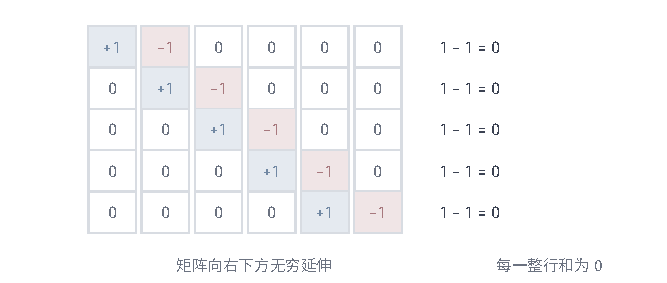
\includegraphics[width=112mm]{figures/01-mathematical-preliminaries-upper/01-mathematical-language-combinatorics-analysis-optimization/tikz/comprehension-additions/fubini-cancellation-grid.pdf}
  \caption{无穷矩阵$a_{i,j}=\mathbb I\{j=i\}-\mathbb I\{j=i+1\}$的左上角，展示前五行、前六列，矩阵向右下方继续。每一整行的和为$0$；第一整列的和为$1$，其他整列的和为$0$。蓝、红单元分别为$+1,-1$，每行绝对和为$2$，因而无穷矩阵不绝对可加。}
  \label{fig:vol1-add-fubini-cancellation-grid}
\end{figure}

$\sigma$有限也有实际作用。在$[0,1]$上让$x$采用Lebesgue测度、$y$采用
定义在所有子集上的计数测度，取非负函数$f(x,y)=\mathbb I\{x=y\}$。
对角线的补集是$[0,1]^2$内的相对开集；由前面实平面开集的可数有理矩形表示，
它是可数个可测矩形的并。因此取补后，对角线属于乘积$\sigma$代数。
先对$y$计数再对$x$积分得到$1$，
先对$x$求长度再对$y$计数却得到$0$。这里不满足本章Tonelli版本的$\sigma$有限条件，
不能只凭非负性换序。

\subsubsection{坐标变换后的积分}
\paragraph{变换前后的区域权重}

前章式~\eqref{eq:analysis-multivariate-change-variables}已经解释坐标变换的两项作用：用$T(\bm x)$改写函数，同时用$|\det\bm J_T(\bm x)|$校正体积。这里保留同一变换，扩大被积函数的范围。因此改变的不是体积规则，而是哪些函数可以使用它。

设$U,V\subseteq\mathbb R^d$为开集，$T:U\to V$是连续可微双射，其逆也连续可微，且Jacobian行列式处处非零。这样的变换及其逆在每个足够小的紧邻域上都是Lipschitz，因而把勒贝格零测集映成零测集；与Borel可测性合并后，能处理完备化增加的可测集合。只知道一般映射可测，尚不足以沿用Jacobian体积公式。

\paragraph{可测与可积条件下的换元}

对非负勒贝格可测函数$g:V\to[0,\infty]$，有
\begin{equation}
 \int_Vg(\bm y)\,\mathrm d\bm y
 =\int_Ug(T(\bm x))|\det\bm J_T(\bm x)|\,\mathrm d\bm x,
\label{eq:measurable-change-variables}
\end{equation}
允许共同值为无穷。若$g$有符号且绝对可积，则先对$|g|$使用非负版本，确认变换后的绝对积分有限，再对正负两部分相减，公式仍成立且取有限值。一般版本由可测集合的体积变换推广到简单函数，再经单调逼近得到；不能仅凭每一点的线性化就完成对一般集合的证明\scite{math-folland1999real}

例如前章的极坐标参数化，需要先删去原点、径向接缝和边界才能满足所用双射版本。这些集合测度为零，补回后不影响非负积分或可积函数的积分。若参数在正测度区域重复覆盖，同一点就会被多次累计，不能继续直接套用这里的公式。

\FloatBarrier
\section{函数逼近与积分的极限}
\label{sec:measurable-convergence-and-integrals}

前章已经区分逐点误差与整个范围上的统一误差。引入测度以后，还可以忽略零测例外，或把误差按权重累计；这些新的比较口径并不等价。本节先建立它们各自比较的对象，再研究单调结构、非负性与共同可积支配怎样保留积分，最后把结论用于参数积分的连续性和求导。贯穿的检验仍是前章的幂函数列和连续尖峰，避免把更换积分定义误认为自动允许交换极限。

\subsection{函数逼近的误差尺度}

按位置比较要求每个输入最终稳定，按积分比较则允许少量区域暂时保留较大误差。下面依次说明零测例外、累计误差和忽略零测例外后的统一误差，明确每一项条件究竟控制什么。

\subsubsection{点态极限与零测修改}
\paragraph{几乎处处收敛}

如果某些输入占零权重，是否必须在它们上面也逼近？积分任务通常不需要，
但必须先固定采用的测度和可忽略的范围。
\begin{definition}[几乎处处收敛]
\label{def:analysis-almost-everywhere-convergence}
给定测度空间$(X,\mathcal A,\mu)$和实函数$f_n,f$，若存在$E\in\mathcal A$、
$\mu(E)=0$，使
\[
 \forall x\in X\setminus E,\quad
 \forall\varepsilon>0,\quad
 \exists N=N(x,\varepsilon),\quad
 \forall n\geq N,\quad |f_n(x)-f(x)|<\varepsilon,
\]
就称$f_n$在$\mu$下几乎处处收敛到$f$。
\end{definition}
这里是先选一个零测集，再在它的补集上逐点收敛；每个精度和每一项不能任意丢掉
不同的正测度区域。可数个零测例外可以取并后统一，任意不可数个零测集的并却未必零测。
例如$x^n$关于$[0,1]$上的Lebesgue测度几乎处处趋于零，虽然它不在$x=1$处趋于零。
又如$f_n(x)=n\mathbb I_{\{0\}}(x)$几乎处处趋于零，但在$0$处连有限极限都没有。
若要求极限仍可测，本章采用各$f_n,f$均可测的版本；在未完备空间中，
不能从几乎处处关系自动推出任意指定的例外点取值可测。

\paragraph{点值读数与积分等价}

固定输入$x_0$处的读数$f(x_0)$，与函数在整个区域上的积分是不同对象。勒贝格测度下，改变单点值不改变积分；计数测度下则会改变累计。例如在$[0,1]$上令$f=0$，$g(0)=100$、其余位置$g=0$，则$\int|f-g|\,\mathrm dx=0$，但两者在零点的读数不同。以后把几乎处处相同的函数合并时，合并的是积分任务中无法区分的对象，不是宣称它们每一点都相等。

\subsubsection{按积分累计的函数误差}
\paragraph{$L^1$、$L^2$与一般$L^p$误差}

如果关心的是按测度累计的误差，就要先说明被比较的函数属于什么空间。
积分不区分只在零测集上不同的可测函数：即使$f$不处处为零，$\int|f|^p\,\mathrm d\mu$
也可能为零。把这类函数视为同一个元素，才能让零误差对应空间中的同一个对象。
我们还希望这项长度满足范数的规则：非负、只在零元素上为零，乘以常数后按其绝对值缩放，
并满足三角不等式。最后一条保证两次误差合并后的长度不超过各自长度之和。
\Needspace{12\baselineskip}
\begin{definition}[$L^p$空间与范数]
\label{def:analysis-lp-space}
设$(X,\mathcal A,\mu)$为测度空间，$1\leq p<\infty$。对可测实函数定义等价关系
\[
  f\sim g\quad\Longleftrightarrow\quad f=g\text{在$\mu$下几乎处处成立}.
\]
$L^p(\mu)$由满足$\int_X|f|^p\,\mathrm d\mu<\infty$的可测实函数的等价类$[f]$组成，
其范数定义为
\[
  \lVert[f]\rVert_{L^p(\mu)}
  =\left(\int_X|f|^p\,\mathrm d\mu\right)^{1/p}.
\]
该值不依赖代表元的选择。下文用代表元$f$代写等价类$[f]$，并简记范数为
$\lVert f\rVert_p$。
\end{definition}

取$p$次根使长度按一次比例缩放：$\lVert af\rVert_p=|a|\lVert f\rVert_p$。$p=1$累计绝对误差，$p=2$累计平方误差后开方，更大的$p$对较大幅度赋予更大权重。这些量首先是函数误差的不同比较方法，尚未涉及导数。

固定这个空间以后，函数列的收敛就可以由累计误差定义。
\begin{definition}[$L^p$收敛]
\label{def:analysis-lp-convergence}
设$1\leq p<\infty$，且$f_n,f\in L^p(\mu)$。若
\begin{equation}
  \lVert f_n-f\rVert_p
  :=
  \left(
    \int_X|f_n-f|^p\,\mathrm{d}\mu
  \right)^{1/p}
  \longrightarrow0,
  \qquad 1\leq p<\infty.
\label{eq:analysis-lp-convergence}
\end{equation}
就称$f_n$在$L^p(\mu)$中收敛到$f$。
\end{definition}

例如$u_n(x)=x^n$关于$[0,1]$上的勒贝格测度几乎处处趋零，而且
\[
 \lVert u_n\rVert_p^p=\int_0^1x^{np}\,\mathrm dx=\frac1{np+1}\longrightarrow0.
\]
它在端点附近始终有接近一的取值，因而不一致趋零。图~\ref{fig:analysis-power-convergence-scales}保留前章的逐点极限代表：该代表在端点一处取一，其余处取零。它与零函数属于同一个几乎处处等价类，故图中的积分误差与上式相同。

\begin{figure*}[htbp]
  \centering
  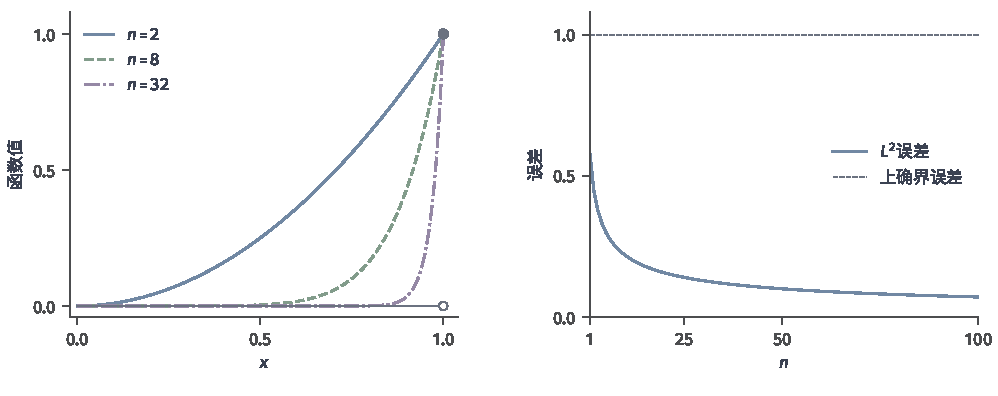
\includegraphics[width=169.0mm]{figures/01-mathematical-preliminaries-upper/01-mathematical-language-combinatorics-analysis-optimization/matplotlib/analysis-power-convergence-scales/figure.pdf}
  \caption{$x^n$在$[0,1]$上的两种整体尺度。左图蓝、绿、紫线分别取$n=2,8,32$；灰线与端点标记表示逐点极限，
 它在$x<1$处为零、在$x=1$处为$1$。右图蓝色曲线为精确的$L^2$误差$(2n+1)^{-1/2}$，
 灰虚线为始终等于$1$的普通上确界误差；单点$x=1$的修改不影响积分。图为解析教学示例。}
 \label{fig:analysis-power-convergence-scales}
\end{figure*}

\paragraph{误差运算与极限存在}

把误差称为范数，还需要能控制误差相加。对$1<p<\infty$，令$q=p/(p-1)$，下面第一式要求$f\in L^p$、$g\in L^q$，第二式要求$f,g\in L^p$。Hölder不等式和Minkowski不等式分别给出
\begin{align}
 \int_X|fg|\,\mathrm d\mu&\leq\lVert f\rVert_p\lVert g\rVert_q,
 \label{eq:measurable-holder}\\
 \lVert f+g\rVert_p&\leq\lVert f\rVert_p+\lVert g\rVert_p.
 \label{eq:measurable-minkowski}
\end{align}
第一式控制乘积累计，第二式控制合并误差。对$p=1$，第二式直接来自逐点三角不等式；第一式的对应版本在$g$本质有界时为$\int|fg|\leq\lVert f\rVert_1\lVert g\rVert_{L^\infty}$，本质有界的定义在下一小小节给出。

Hölder可由非负实数$a,b$的标量不等式$ab\leq a^p/p+b^q/q$得到：当两个范数非零时，先把$f,g$除以各自范数，再对不等式积分，右侧为$1/p+1/q=1$。若某个范数为零，函数几乎处处为零，结论也成立。要得到Minkowski，先用$|f+g|^p\leq2^{p-1}(|f|^p+|g|^p)$确认和属于$L^p$，再写
\[
 \lVert f+g\rVert_p^p
 \leq\int_X(|f|+|g|)|f+g|^{p-1}\,\mathrm d\mu
 \leq(\lVert f\rVert_p+\lVert g\rVert_p)\lVert f+g\rVert_p^{p-1}.
\]
最后一步对两项分别用Hölder；若$\lVert f+g\rVert_p>0$，约去其$p-1$次幂即可。范围$p\geq1$有实际作用：在两点计数测度上，若$0<p<1$，$(1,0)$与$(0,1)$各有长度一，和的长度却是$2^{1/p}>2$，三角不等式失败。

误差还可以在不知道极限时判断：若$\lVert f_n-f_m\rVert_p\to0$于$n,m\to\infty$，就称它为$L^p$柯西列。对$1\leq p<\infty$，每个这样的函数列都有$L^p$极限，即$L^p$完备。下面说明极限如何构造。选子列$f_{n_k}$使$\lVert f_{n_{k+1}}-f_{n_k}\rVert_p\leq2^{-k}$，并令
\[
 H_M=|f_{n_1}|+\sum_{k=1}^M|f_{n_{k+1}}-f_{n_k}|.
\]
由Minkowski，$\lVert H_M\rVert_p\leq\lVert f_{n_1}\rVert_p+1$；由非负单调收敛，$H=\lim_M H_M$属于$L^p$，因而几乎处处有限。在这些位置，相邻差绝对可加，所以$f_{n_k}$逐点收敛到一个可测有限函数$f$；其余可测零测集上令$f=0$。同时$|f|\leq H$几乎处处，故$f\in L^p$。再用相邻差的尾和和单调收敛得到
\[
 \lVert f-f_{n_K}\rVert_p\leq\sum_{k=K}^{\infty}2^{-k}\longrightarrow0.
\]
原列的柯西条件与三角不等式便把子列收敛提升为整列的$L^p$收敛。这个构造保留的是积分误差意义下的极限；后续函数空间章再研究这些空间的结构和算子。

\subsubsection{忽略零测例外后的统一控制}
\paragraph{本质上确界与$L^\infty$误差}

普通上确界会被单个异常点改变，而保持可测性的零测集修改不影响积分。
若仍要控制最坏误差，却允许忽略测度为零的例外，就应比较函数绝对值的本质上界。
\begin{definition}[本质有界与绝对值的本质上界]
\label{def:analysis-essential-bound}
设$(X,\mathcal A,\mu)$为测度空间，$f:X\to\mathbb R$可测。其绝对值$|f|$的
\term{本质上确界}（essential supremum）定义为
\[   \operatorname*{ess\,sup}_{x\in X}|f(x)|   =   \inf\{M\geq0:|f(x)|\leq M\text{几乎处处}\}. \]
若集合中没有有限的$M$，上式取$+\infty$；若上式有限，就称$f$本质有界。
这里衡量的是$|f|$的大小，不是一般有符号函数$f$的本质上确界。
\end{definition}

将本质有界函数按几乎处处相同合并后，本质上界便给出等价类的长度：零长度恰好对应零等价类。
\begin{definition}[$L^\infty$空间与范数]
\label{def:analysis-linfty-space}
在同一测度空间上，$L^\infty(\mu)$由本质有界可测实函数的几乎处处等价类组成，
其范数定义为
\begin{equation}
  \lVert f\rVert_{L^\infty}
  =
  \operatorname*{ess\,sup}_{x\in X}|f(x)|.
\label{eq:analysis-essential-supremum-norm}
\end{equation}
同样用$f$代写等价类$[f]$；该范数不依赖代表元。
\end{definition}
例如在$[0,1]$上使用Lebesgue测度，令$f(0)=100$、其余位置$f(x)=0$，
则普通上确界为$100$，$|f|$的本质上确界却为$0$。
相应地，$\lVert f_n-f\rVert_{L^\infty}\to0$称为$L^\infty$收敛。
对每个$\varepsilon>0$，它要求某个$N$之后的全部误差都在几乎处处意义下
小于$\varepsilon$。可取精度$1/k$，把各$n,k$对应的可测零测例外并为一个零测集$E$；
于是存在同一个$E$，使$f_n$在$X\setminus E$上一致收敛。
反之，这种补集上的一致收敛立即给出$L^\infty$收敛。
因此它蕴含几乎处处收敛，却不一定是原集合上的一致收敛。
上面的$n\mathbb I_{\{0\}}$在$L^\infty$中恒等于零，普通上确界却为$n$。
对$x^n$，本质上确界误差仍为$1$，因为接近$1$的一整段正测度区间保留大误差，
不是删除端点就能消除。

$L^\infty$同样完备。若$f_n$为该范数下的柯西列，对每个精度$1/k$选出尾部范数界，并把可数个函数对及精度对应的可测零测例外取并。其补集上所有相应点值误差共同有界，因而$f_n$是一致柯西列；逐点取极限，例外集上置零，即得到本质有界的可测极限，并在$L^\infty$中收敛。这里沿用前章一致柯西的论证，只是先去掉了同一个零测集。

\paragraph{误差尺度的适用范围}

若$\mu(X)<\infty$且$f_n,f\in L^p$，一致收敛蕴含$L^p$收敛，因为
\[   \lVert f_n-f\rVert_p   \leq   \mu(X)^{1/p}\sup_{x\in X}|f_n(x)-f(x)|. \]
当空间测度无穷时，即使各项仍属于$L^p$，这个推论也可能失败。在$\mathbb R$上采用
Lebesgue测度，固定$1\leq p<\infty$，并取
\[
  f_n(x)=\frac1n\mathbb I_{[0,n^p]}(x).
\]
每个$f_n$都属于$L^p$，且$\sup_x|f_n(x)|=1/n\to0$，所以一致收敛到零；但
\[
  \lVert f_n\rVert_p^p=\frac{n^p}{n^p}=1,
\]
因而不在$L^p$中收敛到零。幅度虽降低，非零区域却同步扩大，累计误差没有随之减小。

反过来，积分误差小也不保证整列在几乎每个点收敛。
\begin{example}[小区间轮流扫过定义域]
\label{ex:analysis-lp-without-ae-limit}
在$[0,1)$上按轮次细分区间，令
\[
 f_{2^k+j}(x)=\mathbb I_{[j2^{-k},(j+1)2^{-k})}(x),
 \qquad k=0,1,\ldots,\quad j=0,\ldots,2^k-1.
\]
第$k$轮依次访问$2^k$个小区间，每个函数的$L^p$范数为$2^{-k/p}$，
所以对每个有限$p\geq1$，$f_n\to0$在$L^p$中成立。
但每个$x\in[0,1)$在每轮恰有一次取值$1$，也在无穷多个其他时刻取值$0$。
因此整列在每个$x$处都不收敛。积分看到每次被访问的区间越来越小，
逐点收敛却要求同一个输入从某一时刻起一直稳定，这两个要求不能互代。
\end{example}

同一组连续尖峰还能检验点值与累计误差的区别。在$[0,1]$上记$t_+=\max\{t,0\}$，令
\begin{equation}
 b_n(x)=(1-|2nx-1|)_+,\qquad a_n(x)=2n\,b_n(x).
\label{eq:measurable-continuous-spikes}
\end{equation}
两列的支撑都为$[0,1/n]$，在零点的值也都是零，因此处处趋零。由三角形面积及换元计算，
\[
 \int_0^1b_n\,\mathrm dx=\frac1{2n},\qquad
 \int_0^1a_n\,\mathrm dx=1,\qquad
 \int_0^1b_n^p\,\mathrm dx=\frac1{n(p+1)}.
\]
于是$b_n$在每个有限$L^p$中趋零，却不在$L^\infty$中趋零；$a_n$甚至不在$L^1$中趋零，且对$p>1$有$\lVert a_n\rVert_p^p=2^pn^{p-1}/(p+1)$。两列都由连续函数组成，失败原因与函数在单点是否跳跃无关。

几乎处处和$L^p$范数还依赖所选测度：换一个测度，原先可忽略的集合可能重新变得重要。
若$Q$对$P$\term{绝对连续}（absolutely continuous），记作$Q\ll P$，则原来$P$
意义下的零测例外在$Q$下仍可忽略；
也就是对任意可测$A$，$P(A)=0$蕴含$Q(A)=0$。
这一测度关系保留的是零测集，不同于前面用距离控制输入、输出变化的映射连续性。
若没有$Q\ll P$，换分布可能给原零测集正质量。例如$P$是$[0,1]$上的均匀分布，
$Q$把全部质量放在$0$点；两个只在$0$处不同的函数在$P$意义下等价，在$Q$意义下
却可能具有完全不同的误差。
即使$Q\ll P$，$L^p$收敛也不能仅凭零测关系转移。令$P$是$(0,1)$上的长度测度，
$Q(A)=\int_A(2\sqrt x)^{-1}\,\mathrm dx$，其总质量为$1$，并有$Q\ll P$。
固定有限$p\geq1$，取$u_n=n^{1/(2p)}\mathbb I_{(0,1/n)}$，则
\[
 \lVert u_n\rVert_{L^p(P)}^p=n^{-1/2}\to0,\qquad
 \lVert u_n\rVert_{L^p(Q)}^p
 =\sqrt n\int_0^{1/n}\frac{\mathrm dx}{2\sqrt x}=1.
\]
$Q$虽没有给$P$零测集新增质量，却更看重靠近$0$的区域。
若另有统一常数$C$使$Q(A)\leq CP(A)$对所有可测$A$成立，
从简单函数经单调逼近可得$\lVert u\rVert_{L^p(Q)}
\leq C^{1/p}\lVert u\rVert_{L^p(P)}$，
此时才有直接的积分误差转移保证。

\subsection{积分交换极限的条件}
\label{sec:analysis-limit-integral-interchange}

前面已看到，处处趋零仍可能保留非零积分。这里固定测度和积分方式，改变对函数列的附加要求：非负递增保留累计量，一般非负列先保留单向界，另有共同可积支配时才能保证更一般的积分交换。每项条件都针对刚才的局部集中或向无穷远处移动的贡献。

\subsubsection{非负函数列的积分极限}
\paragraph{单调逼近中的积分保持}

定理~\ref{thm:analysis-monotone-convergence}已经在积分构造中证明：若非负可测函数几乎处处递增至$f$，其积分也递增至$\int f$，允许无穷值。它不要求一致收敛，也不要求共同可积上界。例如有限有理点集的示性函数递增至有理数集示性函数，各步与极限的积分都是零；在$(0,\infty)$上$\mathbb I_{(0,n)}\uparrow1$，各步积分则从$n$增至无穷。两者同样满足定理，区别在极限总量是否有限。

\paragraph{一般非负逼近中的单向界}

若删除单调要求，只保留非负性，连续尖峰$a_n$说明积分等式可能失败，但仍有一个方向的界。对可能不收敛的函数列，可以用每个位置的下极限比较尾部贡献。

\begin{lemma}[Fatou引理]
\label{lem:analysis-fatou}
若$f_n:X\to[0,\infty]$可测，则
\begin{equation}
  \int_X\liminf_{n\to\infty}f_n\,\mathrm{d}\mu
  \leq
  \liminf_{n\to\infty}\int_Xf_n\,\mathrm{d}\mu.
\label{eq:analysis-fatou}
\end{equation}
\end{lemma}
\begin{proof}
令$g_n=\inf_{k\geq n}f_k$。则$g_n$可测， $0\leq g_n\uparrow\liminf_k f_k$。由单调收敛定理，
\[   \int\liminf_k f_k\,\mathrm{d}\mu   =   \lim_{n\to\infty}\int g_n\,\mathrm{d}\mu. \]
对每个$k\geq n$都有$g_n\leq f_k$，故
\[   \int g_n\,\mathrm{d}\mu   \leq   \inf_{k\geq n}\int f_k\,\mathrm{d}\mu. \]
令$n\to\infty$便得到式~\eqref{eq:analysis-fatou}。
\end{proof}

非负条件也不能直接删除。若改取$u_n=-n\mathbb I_{(0,1/n)}$，则
$\liminf_n u_n=0$处处成立，而$\int u_n=-1$；原不等式会变成错误的$0\leq-1$。
若另有共同的可积下界$h$使$u_n\geq h$，则可以对$u_n-h\geq0$应用Fatou，
再移去有限的$\int h$。可积下界是可用的推广条件，不是无条件允许负值。

Fatou通常只给一个方向。对式~\eqref{eq:measurable-continuous-spikes}中的$a_n$，左边为零、右边为一，不等式严格成立。极限前的累计量集中在越来越小的区域，逐点极限没有保留它。下面图~\ref{fig:analysis-convergence-obstacles}左侧的矩形尖峰提供同样的机制：它与连续三角尖峰的连续性不同，积分失效的原因相同。右侧回顾前章的求导反例，说明积分与导数需要各自的误差控制。

\subsubsection{共同可积控制下的积分交换}
\paragraph{支配收敛与积分误差}

若函数会振荡或有正负值，单调条件未必可用。可以要求同一个非负可积函数$g$控制所有$|f_n|$，让局部高峰和远处尾部都受有限总量限制。每个$f_n$分别可积还不够，下面要求的是一项覆盖整列函数的共同控制。

\begin{theorem}[支配收敛定理]
\label{thm:analysis-dominated-convergence}
设$f_n,f:X\to\mathbb{R}$可测，$f_n\to f$几乎处处，并且存在非负可积函数$g$使
$|f_n|\leq g$几乎处处对所有$n$成立，则$f$可积，而且
\[   \lim_{n\to\infty}\int_Xf_n\,\mathrm{d}\mu   =   \int_Xf\,\mathrm{d}\mu. \]
此外，$\int|f_n-f|\,\mathrm{d}\mu\to0$。
\end{theorem}
\begin{proof}
把收敛或控制条件失效的可测零测集的可数并记为$N$，并将$f_n,f,g$在$N$上都改为
$0$。这些函数仍可测且积分不变，因而下述关系可以按逐点意义使用。
由$|f_n|\leq g$并取逐点极限可得$|f|\leq g$几乎处处，所以$f$可积。函数$g+f_n$与$g-f_n$均非负。对它们分别使用Fatou引理，
\begin{align*}
  \int g+\int f
  &\leq
  \int g+\liminf_{n\to\infty}\int f_n,\\
  \int g-\int f
  &\leq
  \int g-\limsup_{n\to\infty}\int f_n.
\end{align*}
由于$\int g<\infty$，可以从两边减去它，得到
\[   \int f   \leq\liminf_n\int f_n   \leq\limsup_n\int f_n   \leq\int f. \]
故积分收敛到$\int f$。

最后，$|f_n-f|\to0$几乎处处，且 $|f_n-f|\leq2g$。再对非负函数$|f_n-f|$应用刚证明的积分交换结论，得到 $\int|f_n-f|\,\mathrm{d}\mu\to0$。
\end{proof}

\paragraph{同一组函数列的条件核验}

在$[0,1]$上，幂函数列$x^n$几乎处处趋零，且被可积常数一支配，故积分趋零；这与它不一致收敛没有矛盾。连续尖峰$b_n$也满足$0\leq b_n\leq1$，所以支配收敛给出$\int b_n\to0$。面积保持为一的$a_n$则没有共同可积支配，下面直接检查这一缺口。

假设$g\geq a_n$几乎处处对每个$n$成立，将可数个例外并为$N$。对$0<x<1/8$且$x\notin N$，取$n=\lfloor1/(2x)\rfloor$，有$1-2x<2nx\leq1$，因而$b_n(x)\geq1-2x>3/4$；同时$n\geq1/(4x)$。于是
\[
 g(x)\geq a_n(x)=2nb_n(x)\geq\frac{3}{8x}.
\]
右边在零点附近不可积，矛盾。这里并非支配条件暂时没有找到，而是这种可积支配根本不存在。

贡献也可以向无穷远移动：在$\mathbb R$上令$f_n=\mathbb I_{[n,n+1)}$，则处处趋零且积分恒为一。它虽共用常数上界一，那个上界在整条实轴上不可积。相反，$x^n/\sqrt x$在$(0,1)$上由可积的$x^{-1/2}$支配，积分趋零。支配函数可以无界，需要有限的是其累计量。

\begin{figure*}[htbp]
  \centering
  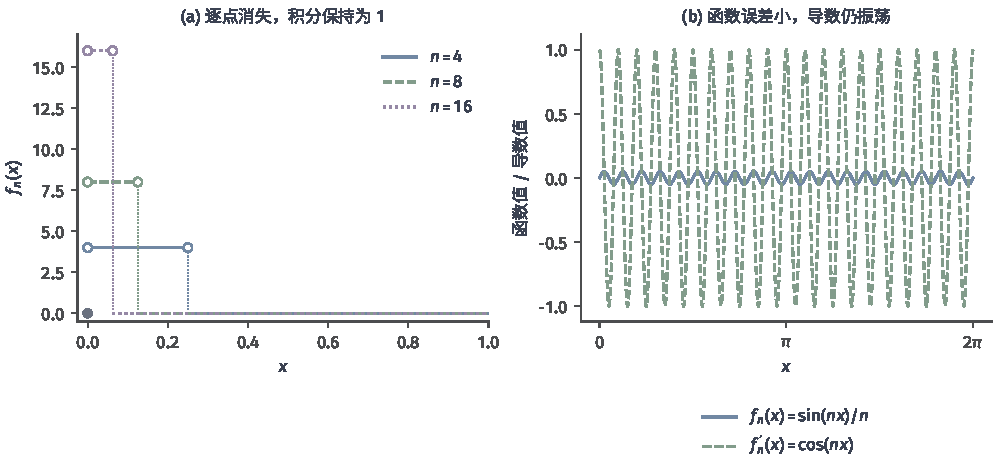
\includegraphics[width=169.0mm]{figures/01-mathematical-preliminaries-upper/01-mathematical-language-combinatorics-analysis-optimization/matplotlib/analysis-convergence-obstacles/figure.pdf}
  \caption{两种交换运算的障碍。左图的尖峰支撑不断收缩，但高度同步增长，每条曲线的积分仍为$1$；开圆点标出不取的上端点，竖虚线仅提示跳跃。右图取$n=20$，$\sin(nx)/n$的函数幅度很小，导数$\cos(nx)$仍有单位幅度。两图均为按给定函数公式构造的教学示例。}
 \label{fig:analysis-convergence-obstacles}
\end{figure*}

表~\ref{tab:analysis-interchange-conditions}汇总各项交换的不同条件。积分等式成立的依据来自这些条件，不能仅由已经存在的点态极限推出。
\begin{table*}[htbp]
 \centering\small
 \begin{tabularx}{\linewidth}{@{}lXX@{}}
 \toprule
 结果 & 核对的条件 & 可得到的结论\\
 \midrule
 单调收敛 & 非负可测函数逐点或几乎处处递增 & 极限与积分相等，允许无穷值\\
 Fatou引理 & 非负可测函数列 & 先取下极限再积分，不超过先积分再取下极限的结果\\
 支配收敛 & 几乎处处收敛，且共用一个可积绝对上界 & 积分可交换极限，并有$\int|f_n-f|\,\mathrm d\mu\to0$\\
 Tonelli定理 & $\sigma$有限乘积测度上的非负可测函数 & 交换积分次序，允许无穷值\\
 Fubini定理 & $\sigma$有限乘积测度上的绝对可积函数 & 交换积分次序，并得到有限积分\\
 \bottomrule
 \end{tabularx}
 \caption{极限与积分、积分与积分之间的交换条件。表中的测度、可测性和统一控制属于结论的假设。}
 \label{tab:analysis-interchange-conditions}
\end{table*}

\subsection{参数积分的变化}

给定参数$\theta$后，$g(\cdot,\theta)$就是一个被积函数；让参数变化，就得到需要交换极限的一族函数。下面先处理参数趋近时积分是否连续，再将参数差商作为被积函数处理求导。积分区域也随参数变化时，还须另计边界贡献。

\subsubsection{参数变化后的积分连续性}
\paragraph{参数趋近与被积函数趋近}

设$I$为实参数区间，$G(\theta)=\int_Xg(x,\theta)\,\mathrm d\mu(x)$。若对几乎每个$x$，$g(x,\theta)\to g(x,\theta_0)$于$\theta\to\theta_0$，便只得到了各位置的极限。要判断$G$是否连续，还要防止参数变化时贡献集中到狭小区域或移向无穷远。

\paragraph{共同支配下的积分连续}

假设存在同一个可测零测集$N$和同一个非负可积函数$h$，使$x\notin N$时$g(x,\cdot)$在$\theta_0$连续，并且$|g(x,\theta)|\leq h(x)$对$\theta_0$某邻域中的全部参数成立。对任意$\theta_n\to\theta_0$，支配收敛给出$G(\theta_n)\to G(\theta_0)$；由极限的序列判据，$G$在$\theta_0$连续。固定$\theta_0>0$时，$g(x,\theta)=e^{-\theta x}$在$[0,\infty)$上由$e^{-\theta_0x/2}$局部支配，所以$G(\theta)=1/\theta$在正参数处连续。控制范围是所考察参数点的邻域，并不要求同一上界覆盖全部参数。

\subsubsection{参数导数与积分交换}
\paragraph{差商极限与导数支配}

给定参数以后，$g(\cdot,\theta)$是一个函数；让参数接近$\theta_0$时，差商形成一族
逼近函数。因此积分号下求导同时使用前章的微分、
第~\ref{sec:analysis-integration-average}节的积分，以及刚证明的支配收敛。
各点偏导数存在只决定差商的逐点极限；用同一可积函数控制整族差商，才给出把这个极限移入积分的充分条件。
这里“同一”的要求比逐点收敛更强：参数不可数，无法像逐点收敛那样对每个参数分别取得例外集
再合并，因此必须一次控制整个参数邻域上的所有差商。


设
\[   G(\theta)=\int_X g(x,\theta)\,\mathrm{d}\mu(x). \]
形式上希望把导数移入积分号：
\[   G'(\theta)   \stackrel{?}{=}   \int_X\frac{\partial g}{\partial\theta}(x,\theta)\,\mathrm{d}\mu(x). \]
真正需要交换的是差商的极限与积分。固定$\theta_0$，设对每个$\theta\in I$，
$x\mapsto g(x,\theta)$可测，其中$I$是包含$\theta_0$的开区间，并且
$g(\cdot,\theta_0)$可积。假设存在一个可测零测集$N$，使每个$x\notin N$处的
$\theta\mapsto g(x,\theta)$在整个$I$内可微；对每个$\theta$，
偏导数作为$x$的函数可测，并且存在非负可积函数$h$使
\begin{equation}
  \left|
    \frac{\partial g}{\partial\theta}(x,\theta)
  \right|
  \leq h(x)
  \quad
  \text{对所有$x\notin N$及所有$\theta\in I$成立},
\label{eq:analysis-parameter-derivative-domination}
\end{equation}
这里$N$和$h$都不能随参数$\theta$改变；参数不可数，不能靠取所有参数例外集的并
自动获得一个零测集。中值定理先给出
$|g(x,\theta)-g(x,\theta_0)|\leq|\theta-\theta_0|h(x)$，
所以$I$中每个$g(\cdot,\theta)$都可积，$G$在邻域内有有限值。
对非零$t$且$\theta_0+t\in I$，令
\[
 q_t(x)=\frac{g(x,\theta_0+t)-g(x,\theta_0)}{t}.
\]
中值定理又给出$|q_t(x)|\leq h(x)$于$X\setminus N$。
差商在那里趋于$\partial g/\partial\theta(x,\theta_0)$。
对任意非零序列$t_n\to0$应用支配收敛，得到同一个积分极限；
由实数极限的序列判据，这就是$t\to0$的双侧极限。因此
\begin{equation}
  G'(\theta_0)
  =
  \int_X
  \frac{\partial g}{\partial\theta}(x,\theta_0)
  \,\mathrm{d}\mu(x).
\label{eq:analysis-differentiate-under-integral}
\end{equation}
条件~\eqref{eq:analysis-parameter-derivative-domination}是一个便于核对的充分条件； 更一般的版本可以直接控制差商，或使用其他一致可积条件。

例如令$g(x,\theta)=e^{-\theta x}$，$x\in[0,\infty)$、$\theta>0$，
并用Lebesgue测度积分。固定$\theta_0>0$后取
$I=(\theta_0/2,3\theta_0/2)$，则
$|\partial_\theta g|=xe^{-\theta x}\leq xe^{-\theta_0x/2}=:h(x)$。
分部积分给出$\int_0^\infty h(x)\,\mathrm dx=4/\theta_0^2<\infty$，
没有需要删除的例外点，故
$G'(\theta_0)=-\int_0^\infty xe^{-\theta_0x}\,\mathrm dx=-1/\theta_0^2$，
与$G(\theta)=1/\theta$的直接求导一致。
若把参数范围放大到任意接近零的正数，便不能沿用这个固定的控制函数；
交换结论所需的是所考察参数点附近的统一控制。

\begin{example}[参数积分中的控制函数失效]
\label{ex:analysis-parameter-integral-failure}
下面考察参数域边界处对应的右求导问题。对$\theta\geq0$与$x\in(0,1)$，定义
\[   g(x,\theta)   =
\begin{cases}     \dfrac{\theta x}{x^2+\theta^2}, & \theta>0,\\[5pt]     0, & \theta=0.
\end{cases} \]
在$\theta=0$处，对每个固定$x>0$，关于$\theta$的右偏导数都等于$1/x$，但$1/x$在$(0,1)$上不可积。
直接积分得到
\[   G(\theta)   =   \frac{\theta}{2}   \log\left(\frac{1+\theta^2}{\theta^2}\right)   \quad(\theta>0),   \qquad G(0)=0. \]
于是$G(\theta)/\theta$在$\theta\downarrow0$时发散，$G$在$0$处没有有限右导数。积分内的
逐点右导数虽然存在，却缺少统一可积控制；因此这里不能交换右求导与积分。
\end{example}

\paragraph{积分范围变化与边界项}

前面的差商固定了积分区域。如果端点也变化，即使被积函数不依赖参数，积分仍然会变化。例如$G(\theta)=\int_0^\theta1\,\mathrm dx=\theta$的导数为一，而对被积函数求参数偏导只能得到零。

在一维，若$a(\theta),b(\theta)$可微、$a(\theta)<b(\theta)$，且$g(x,\theta)$与$\partial_\theta g(x,\theta)$在包含邻近全部积分区间的紧矩形上连续，则
\begin{equation}
 \frac{\mathrm d}{\mathrm d\theta}\int_{a(\theta)}^{b(\theta)}g(x,\theta)\,\mathrm dx
 =\int_{a(\theta)}^{b(\theta)}\partial_\theta g(x,\theta)\,\mathrm dx
 +g(b(\theta),\theta)b'(\theta)-g(a(\theta),\theta)a'(\theta).
\label{eq:measurable-moving-boundary-integral}
\end{equation}
把积分差拆为固定旧区间内的函数变化、上端新增段和下端移去段，分别除以参数增量取极限，就得到这三项。采用紧矩形上的连续性，是一组便于核对的充分条件；一般可测函数还需保证相应的边界取值与极限有意义，不能仅凭几乎处处等价类指定任意端点读数。

\FloatBarrier
\section{函数的微分与积分恢复}
\label{sec:measurable-differentiation-recovery}

可测函数可以按取值累计，却可能在每一点跳变，不能仅凭可测性讨论经典导数。本节先增加局部Lipschitz条件，回答原函数何时几乎处处可微，并补全前章尖点处的广义变化。随后转向两项互逆的问题：从可积函数形成累计量后，求导能否恢复局部数值；已知函数导数后，积分能否恢复原来的全部变化。后一个方向需要绝对连续性，单有几乎处处导数并不够。

\subsection{函数本身的微分存在}

前章的绝对值函数在零点没有唯一斜率，其他位置仍有经典导数。这里先说明这种“例外可忽略”的结论需要什么变化控制，再研究例外位置能够采用怎样的斜率集合。它们描述的是原函数的变化，不为算法自行指定的反向信号提供精确导数身份。

\subsubsection{局部Lipschitz条件下的可微性}
\paragraph{几乎处处可微的条件}

前章的局部Lipschitz条件要求每个位置附近存在有限常数$L$，使$|f(\bm x)-f(\bm y)|\leq L\lVert\bm x-\bm y\rVert_2$。这比连续性增加了线性幅度控制，但仍允许绝对值那样的尖点。\term{Rademacher定理}（Rademacher theorem）说明，在有限维欧氏空间中，无法形成一阶线性模型的位置只能占零测范围。
\begin{theorem}[Rademacher定理]
\label{thm:measurable-rademacher}
设$U\subseteq\mathbb R^d$为开集，$f:U\to\mathbb R$局部Lipschitz，则$f$关于$d$维勒贝格测度几乎处处全微分存在。即对几乎每个$\bm x\in U$，存在向量$\nabla f(\bm x)$使
\[
 f(\bm x+\bm h)-f(\bm x)-\nabla f(\bm x)^\top\bm h=o(\lVert\bm h\rVert_2).
\]
\end{theorem}
局部版本可用可数个具有Lipschitz界的邻域覆盖$U$，再合并它们的零测例外；定理的核心是Lipschitz控制怎样保证各方向最终组成共同的线性近似。它并非只声明偏导数存在，完整证明需要额外的测度估计\scite{math-simon2014geometric}

\paragraph{例外点与经典导数的边界}

一元函数$|x|$与$\max\{0,x\}$满足Lipschitz条件，各自只在零点不可微；有限段分段线性函数的折点同样是零测例外。多元分段仿射函数在每块内部有固定梯度，块的接合处可能不唯一。几乎处处可微没有在接合处指定某一个梯度，因而不能单凭这项结论确定算法在那里如何更新。

相反，有理数集示性函数虽然可测且可积，却处处不连续，因而处处不可微。阈值函数$\mathbb I\{x\geq0\}$几乎处处导数为零，在跳点不连续；它不满足跳点附近的局部Lipschitz条件。这两个例子分别说明可测性不保证微分，而几乎处处导数也可能没有记录跨越跳点的输出变化。

\subsubsection{不可微位置的广义变化}
\label{sec:analysis-nonsmooth-surrogate-gradient}
\paragraph{邻近可微点的梯度极限}

局部Lipschitz函数在几乎每个邻近位置有梯度，而且邻域内的梯度大小受Lipschitz常数控制。因此可以收集这些梯度趋向当前点时出现的极限，再容纳它们的加权平均。非负权重且权重和为一的有限平均称为凸组合；纳入全部凸组合及其极限得到闭凸包。这个过程保留多种局部斜率，不强行选出唯一导数。

\begin{definition}[Clarke广义梯度]
\label{def:analysis-clarke-generalized-gradient}
设$U\subseteq\mathbb{R}^d$为开集，$f:U\to\mathbb{R}$局部Lipschitz。对内点
$\bm{x}\in U$，$f$在$\bm{x}$处的\term{Clarke广义梯度}（Clarke generalized gradient）定义为
\[
  \partial^\circ f(\bm{x})
  =
  \overline{\operatorname{conv}}
  \left\{
    \lim_{k\to\infty}\nabla f(\bm{x}_k):
    \begin{array}{l}
      \bm{x}_k\in U,\quad\bm{x}_k\to\bm{x},\\
      f\text{在每个 }\bm{x}_k\text{处可微},\\
      \text{且上述梯度极限存在}
    \end{array}
  \right\}.
\]
其中$\operatorname{conv}$表示取所有有限凸组合，横线表示在$\mathbb{R}^d$中取闭包，
即把集合内序列的所有极限点也纳入。
\end{definition}


同一个集合也可以由移动基点的方向差商刻画。对方向$\bm v$，令
\[
 f^\circ(\bm x;\bm v)=\limsup_{\substack{\bm y\to\bm x\\t\downarrow0}}
 \frac{f(\bm y+t\bm v)-f(\bm y)}t.
\]
差商不仅从固定$\bm x$出发，还允许起点$\bm y$从附近趋近。对局部Lipschitz函数，$\partial^\circ f(\bm x)$恰好由满足$\bm g^\top\bm v\leq f^\circ(\bm x;\bm v)$对所有方向$\bm v$成立的向量组成。于是一个表述收集邻近梯度，另一个表述直接限制各方向差商；二者刻画相同的Clarke广义梯度\scite{math-clarke1990optimization}
对连续可微函数，它退化为只含$\nabla f(\bm x)$的单点集；仅在当前点可微时，仍须检查邻近斜率是否稳定，不能一概声称退化为单点。

\paragraph{广义驻点与极值判断}

在原点，$|x|$邻近可微点的梯度为$-1$或$1$，$-|x|$则把这两个斜率的位置交换；两者的Clarke广义梯度都是$[-1,1]$。广义梯度含零只能表示相应驻点条件，不能区分极小与极大。对凸函数，还可以要求候选斜率给出全域的仿射下界：$\bm g$为当前点$\bm x$的凸次梯度，是指
\[
 f(\bm y)\geq f(\bm x)+\bm g^\top(\bm y-\bm x)
 \quad\text{对定义域中每个$\bm y$成立}.
\]
这里凸函数的定义是沿任意线段不高于端点的线性插值：$f((1-t)\bm x+t\bm y)\leq(1-t)f(\bm x)+tf(\bm y)$，其中$0\leq t\leq1$，且定义域包含相应线段。局部Lipschitz凸函数的Clarke广义梯度与这项凸次梯度集合一致；对于一般非凸函数，邻近斜率的闭凸包不再保证全域下界。

例如$f(x)=-|x|$在原点左右两侧的导数分别为$1$与$-1$，故其Clarke广义梯度
是$[-1,1]$，包含零；然而原点是局部最大点。若把凸次梯度的全局下界判据用于原点，就要求$-|y|\geq gy$对所有$y$成立。
当$y>0$时，除以$y$得到$g\leq-1$；当$y<0$时，除以负数使不等号反向，得到$g\geq1$。因此不存在满足条件的$g$。
同样的候选区间$[-1,1]$，在$|x|$上可以刻画全局最小点，在$-|x|$上却不提供这样的
保证。这说明广义梯度中含零只是相应的驻点条件，仍要核对所用定义和函数结构。
图~\ref{fig:analysis-clarke-stationarity-boundary}选取两者共有的候选$g=0$。
在$|x|$中，它给出有效的全局下界；在$-|x|$中，原函数反而处处不高于这条线。
局部斜率的凸包抹去了两边斜率出现的次序，不能替代函数整体上下关系。
\begin{figure*}[htbp]
  \centering
  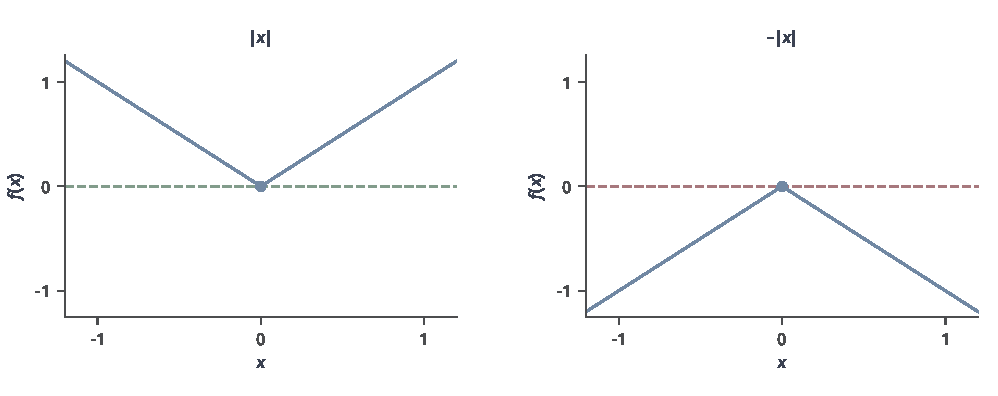
\includegraphics[width=169.0mm]{figures/01-mathematical-preliminaries-upper/01-mathematical-language-combinatorics-analysis-optimization/matplotlib/analysis-clarke-stationarity-boundary/figure.pdf}
  \caption{同一广义驻点条件的不同含义。蓝线分别为$|x|$与$-|x|$，虚线为原点处候选斜率$g=0$对应的直线，左图用绿色，右图用红色。
 两图在原点的Clarke广义梯度均为$[-1,1]$，却分别形成局部最小点与局部最大点；只有左图绿线是全局仿射下界。
 两图共用坐标尺度，由解析式生成。}
 \label{fig:analysis-clarke-stationarity-boundary}
\end{figure*}



在含阈值或脉冲事件的模型中，常保留离散前向映射，却在反向计算时把其导数替换成某个平滑且非零的函数。这种信号称为\term{替代梯度}（surrogate gradient）。它是算法人为指定的近似更新方向，不自动等于前向映射的经典导数，也通常不满足凸次梯度的不等式。因此使用时应分别写清前向函数、反向替代函数及其尺度，不能把训练规则描述成对原离散函数的精确求导。

中心差分
\[   \frac{f(x+\varepsilon)-f(x-\varepsilon)}{2\varepsilon} \]
检验的是实际代入的函数$f$在尺度$\varepsilon$上的变化。若前向计算采用离散函数，反向计算另行指定平滑信号，差分与反向信号就对应不同对象。核验程序时，应分别检查离散前向函数是否正确，以及反向信号是否符合指定的学习规则；不能把二者相等作为未经说明的检验标准。

\subsection{积分累计后的局部恢复}

现在不直接要求被积函数光滑，而从局部可积函数$f$出发，考察小范围内的平均和沿区间形成的累计函数。积分可以抹平零测集上的点值差别，因此期待的恢复结论也只能在几乎处处意义下成立。

\subsubsection{局部平均能否恢复函数值}
\paragraph{邻域缩小时的平均值}

若$f$在$\bm x$连续，则小球中所有函数值都接近$f(\bm x)$，所以小球平均也接近它。对不连续但局部可积的函数，不能再使用所有位置的统一误差，却仍可研究平均误差。这里局部可积是指$U\subseteq\mathbb R^d$内每个紧子集$K$都满足$\int_K|f|\,\mathrm d\bm x<\infty$，记作$f\in L^1_{\mathrm{loc}}(U)$。它允许函数在整个无界区域的绝对积分无穷，只要求每个有限局部累计有意义。

以$B(\bm x,r)$表示欧氏开球，$m_d(B(\bm x,r))$表示其体积。平均
\[
 A_rf(\bm x)=\frac1{m_d(B(\bm x,r))}\int_{B(\bm x,r)}f(\bm y)\,\mathrm d\bm y
\]
比较的是整个邻域的贡献除以邻域体积。半径减小后，问题是这些平均能否读出中心处的值，而不是函数本身是否存在导数。

\paragraph{几乎处处的局部恢复}

勒贝格积分不仅扩大了累计范围，也使局部平均具有以下恢复性质，称为\term{Lebesgue微分定理}（Lebesgue differentiation theorem）\scite{math-hunter2011measure}
\begin{theorem}[Lebesgue微分定理]
\label{thm:measurable-lebesgue-differentiation}
若$f\in L^1_{\mathrm{loc}}(U)$，其中$U\subseteq\mathbb R^d$为开集，则对几乎每个$\bm x\in U$，
\begin{equation}
 \lim_{r\downarrow0}\frac1{m_d(B(\bm x,r))}
 \int_{B(\bm x,r)}|f(\bm y)-f(\bm x)|\,\mathrm d\bm y=0.
\label{eq:measurable-lebesgue-point}
\end{equation}
因此$A_rf(\bm x)\to f(\bm x)$几乎处处。
\end{theorem}
满足式~\eqref{eq:measurable-lebesgue-point}的位置称为勒贝格点。后一结论由$|A_rf(\bm x)-f(\bm x)|$不超过该平均绝对误差得到。一般证明要用覆盖估计控制“某个小球平均误差仍大”的点集，本章使用定理的结论，完整证明见所引教材和讲义。它没有断言$f$在这些点连续或可微。

例如有理数集示性函数的每个区间积分都为零，所有小球平均都为零。它在无理点满足恢复结论，在有理点则不恢复原来取一的读数；有理点恰是零测例外。这说明平均恢复由几乎处处等价类决定，无法检测预先放在零测集上的特殊点值。

\subsubsection{累计函数能否恢复被积函数}
\paragraph{积分上限变化后的导数}

设$f\in L^1([a,b])$，定义$F(x)=\int_a^xf(t)\,\mathrm dt$。对内点$x$及非零增量$h$，$F$的差商就是邻近短区间的平均。若$x$是$f$的勒贝格点，则
\[
 \left|\frac{F(x+h)-F(x)}h-f(x)\right|
 \leq\frac1{|h|}\int_{\min\{x,x+h\}}^{\max\{x,x+h\}}|f(t)-f(x)|\,\mathrm dt.
\]
该单侧短区间包含在$(x-|h|,x+|h|)$中，右侧不超过对称区间平均绝对误差的两倍，故趋零。因此
\begin{equation}
 F'(x)=f(x)\quad\text{对几乎每个$x\in(a,b)$成立}.
\label{eq:measurable-indefinite-integral-derivative}
\end{equation}
这一步用局部平均恢复直接证明累计函数的几乎处处导数，而不要求被积函数先连续。

\paragraph{经典基本定理的扩展范围}

前章对连续被积函数得到每个内点的$F'=f$；这里将对象扩大到全部勒贝格可积函数，结论相应变成几乎处处成立。若$f=\mathbb I_{\mathbb Q\cap[a,b]}$，累计函数$F$恒为零，导数也处处为零，与$f$只在零测集上不同。若$f$是阶跃函数，$F$是折线，折点处未必可导，其他位置仍恢复相应的常数斜率。扩大积分范围并没有为每个指定例外点补上经典导数。

\subsection{导数累计后的整体恢复}

已经知道“可积函数的累计量几乎处处以它为导数”，还不能直接反过来断言“凡是几乎处处有导数的函数，都等于该导数的积分”。函数的全部变化可能有一部分没有被几乎处处导数记录。下面先规定足以排除这种遗漏的绝对连续性，再用康托尔函数说明缺少它会发生什么。

\subsubsection{绝对连续函数的积分表示}
\paragraph{短区间总长度与总变化}

普通连续性控制一个足够短的区间，一致连续性使用共同的长度阈值。现在同时取有限多个不重叠短区间，要求它们的总长度很小时，函数在这些区间上的总变化也很小。这是比一致连续更强的控制：允许区间数增加，不能把有限变化累计到越来越短的总范围中。
\begin{definition}[绝对连续函数]
\label{def:measurable-absolutely-continuous-function}
函数$F:[a,b]\to\mathbb R$称为\term{绝对连续函数}（absolutely continuous function），若对每个$\varepsilon>0$都存在$\delta>0$，使任意有限个内部两两不交的子区间$[a_j,b_j]\subseteq[a,b]$满足
\[
 \sum_j(b_j-a_j)<\delta
 \quad\Longrightarrow\quad
 \sum_j|F(b_j)-F(a_j)|<\varepsilon.
\]
\end{definition}
只取一个区间便得到一致连续。若$F$是$L$-Lipschitz，则总变化不超过$L\sum_j(b_j-a_j)$，所以在紧区间上Lipschitz蕴含绝对连续。但反向不成立：$F(x)=\sqrt x$在$[0,1]$上绝对连续，导数$1/(2\sqrt x)$可积，却没有覆盖零点邻域的有限Lipschitz常数。这里函数的绝对连续控制区间总变化；前面$Q\ll P$是两个测度的零测关系，虽然名称相近，承载对象与定义不同。

\paragraph{常数加可积导数的累计}

绝对连续性恰好给出紧区间上一维函数由可积导数恢复的条件\scite{math-folland1999real}
\begin{theorem}[绝对连续函数的微积分基本定理]
\label{thm:measurable-absolute-continuity-ftc}
函数$F:[a,b]\to\mathbb R$绝对连续，当且仅当存在$g\in L^1([a,b])$使对每个$x\in[a,b]$都有
\begin{equation}
 F(x)=F(a)+\int_a^xg(t)\,\mathrm dt.
\label{eq:measurable-absolute-continuity-representation}
\end{equation}
此时$F'$几乎处处存在，$F'=g$几乎处处，因而$F'$可积且$F(b)-F(a)=\int_a^bF'(t)\,\mathrm dt$；未定义的导数在零测例外上取零不影响积分。
\end{theorem}
从积分表示到绝对连续可以直接核对。取$M>0$，对总长度很小的区间并集$E$，有
\[
 \sum_j|F(b_j)-F(a_j)|\leq\int_E|g|
 \leq M\,m(E)+\int_{\{|g|>M\}}|g|.
\]
先选$M$使尾部积分小于$\varepsilon/2$，再要求$m(E)<\varepsilon/(2M)$，就控制了总变化；尾部能趋零由$|g|$可积及支配收敛保证。导数恢复则已由式~\eqref{eq:measurable-indefinite-integral-derivative}证明。反向的实质是绝对连续排除了集中在零测集上的剩余变化，保证能够找到这样的可积$g$；完整证明需进一步的单调函数或测度分解理论，见所引教材。这里不把一个方向的计算当成全部等价关系的证明。

\subsubsection{几乎处处导数不足以恢复的情形}
\paragraph{康托尔函数的非零变化}

从$[0,1]$中不断去掉每个剩余闭区间的中间三分之一，得到康托尔集$C$。第$n$步剩下$2^n$个长度$3^{-n}$的区间，总长度为$(2/3)^n$，因此$m(C)=0$。相应地构造连续非减函数$F_n$：它在已经移去的开区间上恒定，在每个第$n$步保留区间上作线性上升，并使每个保留区间两端的函数值增加$2^{-n}$，总端点值固定为$F_n(0)=0$、$F_n(1)=1$。

进一步细分一个保留区间时，函数值始终留在其两端值之间，故对$m\geq n$有$\sup_x|F_m(x)-F_n(x)|\leq2^{-n}$。于是$F_n$一致收敛到连续函数$F$，称为\term{康托尔函数}（Cantor function）。它在每个被移去的开区间上恒定，因而在$[0,1]\setminus C$的内点导数为零；这些位置覆盖几乎整个区间。所以$F'=0$几乎处处，却有
\[
 \int_0^1F'(x)\,\mathrm dx=0,\qquad F(1)-F(0)=1.
\]
这里的导数在例外位置可取零作为可积代表。失败的不只是处处可导：即使函数连续、几乎处处导数存在且该导数可积，也仍不能恢复全部变化。

\paragraph{导数存在、可积与恢复条件}

康托尔函数为什么不满足绝对连续？取第$n$步的$2^n$个保留区间，它们的总长度$(2/3)^n$趋零，但各区间端点差均为$2^{-n}$，总变化始终为一。这直接违反定义中对总长度与总变化的共同控制。普通连续性乃至一致连续性都没有排除这种行为。

因此需要分别核对三件事：导数是否几乎处处存在、导数的绝对值能否累计、原函数的全部变化是否都由该累计表示。绝对连续给出三者之间的完整联系；仅取前两项仍会遗漏康托尔函数的变化。弱导数、Sobolev与有界变差理论会采用其他方式记录或限制这些变化，完整结构留到第~\ref{chap:functional-analysis-and-approximation}章。

\Needspace{6\baselineskip}
\section{本章小结}
\label{sec:measurable-summary}

测度规定集合的权重，可测性保证按函数取值划出的区域可以测量。由简单函数下逼近建立的勒贝格积分，既保留有限加权和及黎曼积分的共同结果，也容纳有理数集示性函数这类处处不连续的可积对象。有符号累计仍要检查正负部分，得到有限积分需要绝对可积；条件收敛的反常积分不能直接混入这一范围。

扩大积分对象后，函数列的极限仍须单独控制。几乎处处收敛允许零测例外，$L^p$收敛衡量累计误差，$L^\infty$收敛控制忽略零测例外后的统一误差。非负单调结构保留递增累计，一般非负列由Fatou得到单向界，共同可积支配才使更一般的极限与积分交换。连续尖峰$b_n$与$a_n$都处处趋零，积分表现不同的原因在贡献大小及其共同控制，而不在它们是否连续。

微分与积分的关系也有两个方向。局部Lipschitz函数几乎处处可微，Clarke广义梯度则为例外位置保留多种邻近斜率；可测性本身不给出这些微分结论。局部可积函数可以由小范围平均几乎处处恢复，其累计函数也几乎处处恢复被积函数。反过来，由导数恢复原函数的全部变化需要额外条件；一维紧区间上的绝对连续性给出精确的积分表示，康托尔函数说明几乎处处有可积导数仍然不够。
